%% LyX 2.2.1 created this file.  For more info, see http://www.lyx.org/.
%% Do not edit unless you really know what you are doing.
\documentclass[review]{elsarticle}
\usepackage[latin9]{inputenc}
\usepackage{color}
\usepackage{array}
\usepackage{verbatim}
\usepackage{float}
\usepackage{url}
\usepackage{multirow}
%\usepackage{algorithm}
\usepackage{algpseudocode}
\usepackage{amsmath}
\usepackage{amsthm}
\usepackage{graphicx}
\usepackage{amssymb}
\usepackage{amstext}
\usepackage[ruled,vlined,linesnumbered]{algorithm2e}


\makeatletter

%%%%%%%%%%%%%%%%%%%%%%%%%%%%%% LyX specific LaTeX commands.
\DeclareFontEncoding{LGR}{}{}
\DeclareRobustCommand{\greektext}{%
  \fontencoding{LGR}\selectfont\def\encodingdefault{LGR}}
\DeclareRobustCommand{\textgreek}[1]{\leavevmode{\greektext #1}}
\ProvideTextCommand{\~}{LGR}[1]{\char126#1}

\newcommand{\lyxmathsym}[1]{\ifmmode\begingroup\def\b@ld{bold}
  \text{\ifx\math@version\b@ld\bfseries\fi#1}\endgroup\else#1\fi}
  
 \DeclareMathOperator*{\argmax}{arg\,max}
 
 \newcommand{\lyxdot}{.}


\newcommand{\tstart}{\textrm{start}}
\newcommand{\tend}{\textrm{end}}
\newcommand{\tmedian}{\textrm{median}}

%% Because html converters don't know tabularnewline
\providecommand{\tabularnewline}{\\}

%%%%%%%%%%%%%%%%%%%%%%%%%%%%%% Textclass specific LaTeX commands.
  \theoremstyle{definition}
  \newtheorem{defn}{\protect\definitionname}

%%%%%%%%%%%%%%%%%%%%%%%%%%%%%% User specified LaTeX commands.

\usepackage[margin=1in]{geometry}
\newcommand{\subfour}[1]{\vspace*{3mm}{\noindent\bf #1}} 
\newcommand{\subsubfour}[1]{\vspace*{1mm}{\noindent\bf #1}}

\@ifundefined{showcaptionsetup}{}{%
 \PassOptionsToPackage{caption=false}{subfig}}
\usepackage{subfig}
\makeatother

  \providecommand{\definitionname}{Definition}

\begin{document}
\begin{frontmatter}

%\dochead{} %% Use \dochead if there is an article header, e.g., \dochead{Short communication} %\title{Detection of Low-Quality Records in Bioinformatics Sequence Databases by Automated Literature Analysis}
%\title{Automated Detection of Records Inconsistent with the Literature in Bioinformatics Sequence Databases}

\title{Relevance- and Interface-driven Clustering for Visual Information Retrieval} 

%% use optional labels to link authors explicitly to addresses: 
%% \author[label1,label2]{<author name>}
%% \address[label1]{<address>}
%% \address[label2]{<address>}

\author[deakin]{Mohamed Reda Bouadjenek\corref{cor1}}
\ead{reda.bouadjenek@deakin.edu.au}  
\author[UofT]{Scott Sanner}
\ead{ssanner@mie.utoronto.ca}
\author[UofT]{Yihao Du}
\ead{duyihao@mie.utoronto.ca} 


\address[deakin]{School of Information Technology, Deakin University, Waurn Ponds Campus, Geelong, VIC 3216, Australia}

\address[UofT]{Department of Mechanical and Industrial Engineering, The University of Toronto, Canada}

\cortext[cor1]{This work has been primarily completed while the author was at the University of Toronto.} 

\newtheorem{assumption}{\textbf{Assumption}}

\begin{abstract}
Search results of spatio-temporal data are often displayed on a map, but when the number of matching search results is large, it can be time-consuming to individually examine all results, even when using methods such as filtered search to narrow the content focus.  This suggests the need to aggregate results via a clustering method.  However, standard unsupervised clustering algorithms like $K$-means (i) ignore relevance scores that can help with the extraction of highly relevant clusters, and (ii) do not necessarily optimize search results for purposes of visual presentation.  In this article, we address both deficiencies by framing the clustering problem for search-driven user interfaces in a novel optimization framework that (i) aims to maximize the relevance of aggregated content according to cluster-based extensions of standard information retrieval metrics and (ii) defines clusters via constraints that naturally reflect interface-driven desiderata of spatial, temporal, and keyword coherence that do not require complex ad-hoc distance metric specifications as in $K$-means.  %While a globally optimal solution to this novel clustering optimization problem is NP-Hard, we develop fast greedy algorithms that can approximately optimize this objective for real-time search.  
After comparatively benchmarking the new algorithm we propose in offline experiments, we undertake a user study with 24 subjects to evaluate whether this new relevance-driven clustering method improves human performance on visual search tasks in comparison to $K$-means clustering and a filtered search baseline.  Our results show that (a) our greedy optimization approach is fast, near-optimal, and extracts higher-relevance clusters than $K$-means, and (b) these higher-relevance clusters that have been optimized w.r.t. user interface display constraints result in faster search task completion \textcolor{red}{with a high accuracy while requiring a minimum workload for optimal effectiveness and efficiency, and full satisfaction.}



%lower perceived workload, higher perceived usability, and overall stronger user preference vs. comparison methods.

\end{abstract}
\begin{keyword}
Visual Information Retrieval; Relevance-driven Clustering; Visual Search User Study; Clustering via Filter Optimization.
\end{keyword}

\end{frontmatter}

\section{Introduction}

Search results of spatio-temporal data are often displayed on a map or other visual interface~\cite{Teitler2008,Sankaranarayanan2009,Magdy2014,Ghanem2014,ANDRIENKO2016172,Eldawy2016}.  However, given the massive volume of available information in many applications (e.g., thousands of geolocated tweets matching a query), displaying all relevant results would often result in a saturated and unreadable display~\cite{Landesberger2011,Liu2014,Sun2013}.

In many settings, it is natural to assume that search results  cluster into spatially, temporally, and topically related content that can be aggregated and presented as a single unit rather than individual results~\cite{Manning2008}.  
Such approaches leverage the \emph{cluster hypothesis} of Information Retrieval (IR)~\cite{Salton1971,Jardine1971,Voorhees1985,Manning2008}, which posits that documents in the same cluster should behave \emph{similarly} with respect to information needs. 

\begin{figure*}[t]
\begin{centering}
\subfloat[Baseline display showing all results.]{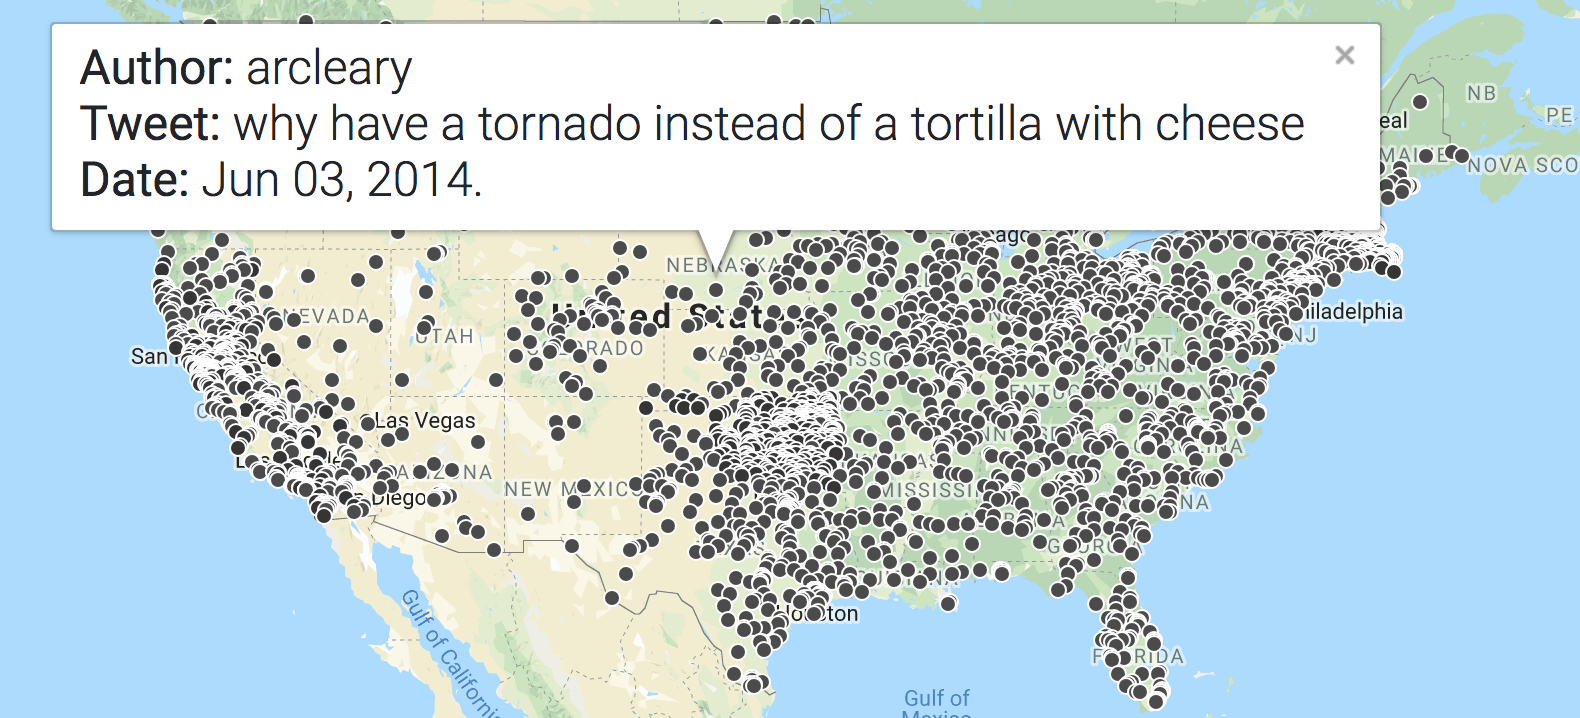
\includegraphics[width=8cm]{baseline}\label{Fig:GlobalDisplay}}\hspace{0.09cm}
\subfloat[K-means based clustered results.]{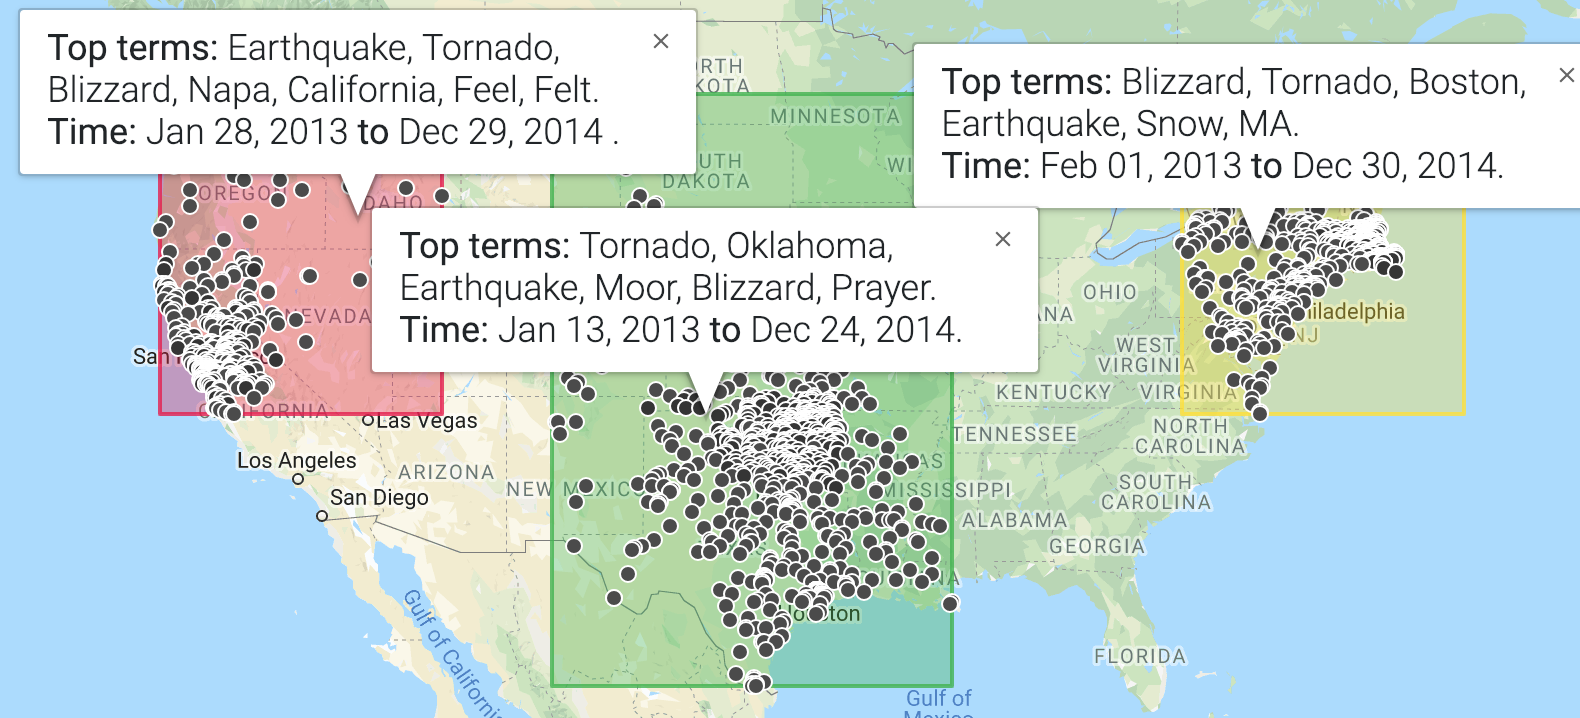
\includegraphics[width=8cm]{kmeans3}\label{Fig:KMeans_FilteredDisplay}}\hspace{0.09cm}
\subfloat[Relevance-driven clustered results.]{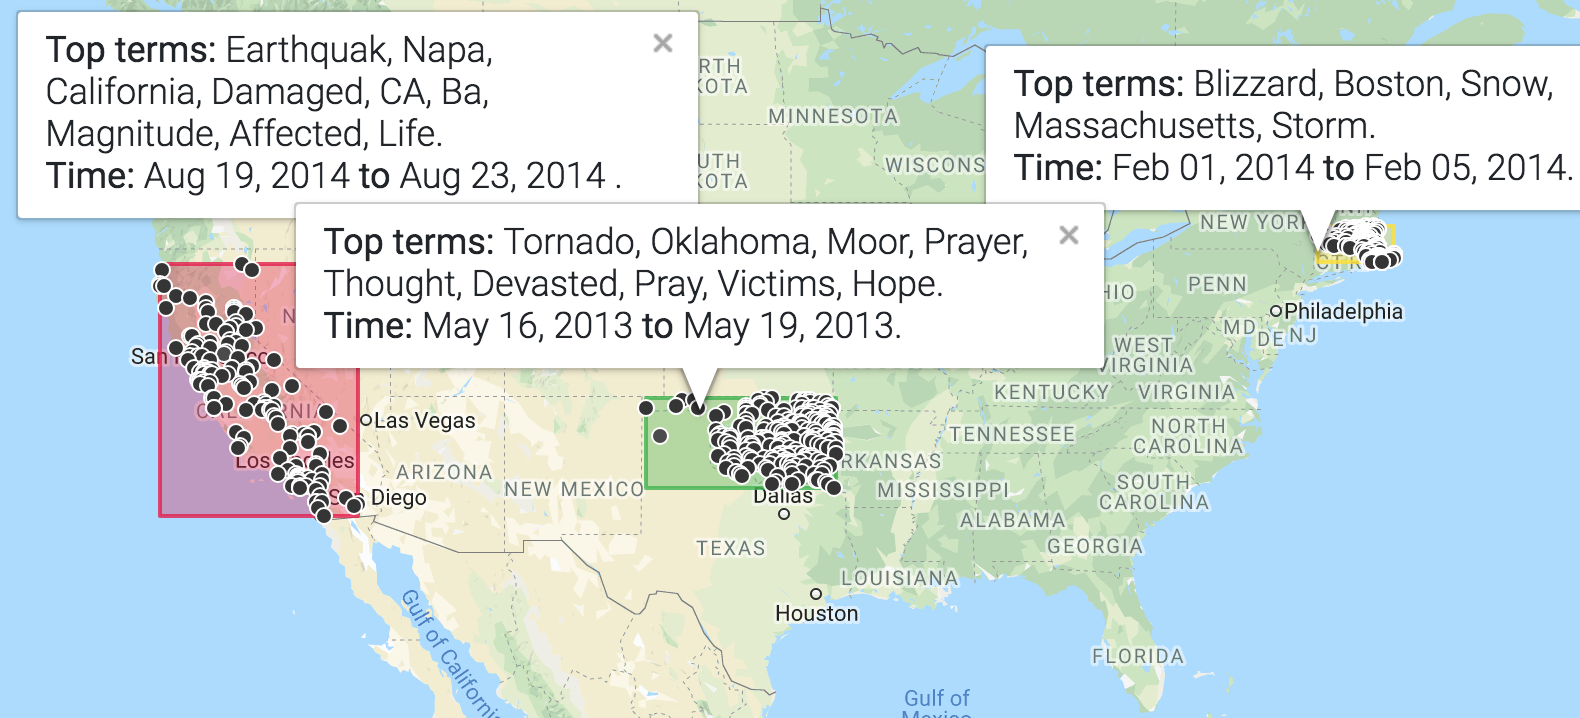
\includegraphics[width=8cm]{bps}\label{Fig:BPS_FilteredDisplay}}
\par\end{centering}
\caption{(a)~An interface for visual information retrieval in a multiyear Twitter corpus showing \emph{all} geolocated tweets that match a query related to natural disasters.
%the query ``tornado, blizzard, earthquake''.
(b)~A $K$-means clustered version of the \emph{same} matching search results, but only showing the \emph{top three} clusters of tweets delineated by bounding boxes.  Since $K$-means uses a compound distance metric that must trade off distance in time, space, and keyword content, its clusters often include unrelated content that is further exacerbated by the fact that $K$-means does not take into account relevance scores of content w.r.t. the query.  For these reasons, while $K$-means does manage to find reasonable clusters in the data, one can see that the spatial and content coherency of the clusters can be improved.
%may vary widely in the clusters since $K$-means ignores 
%Because some matching search results are more relevant than others, the coherence of clusters is corrupted which limits their utility to extract information regarding the events related to the query -- the bounding box defined by each cluster is too wide to clearly identify the location of each event (e.g., the large bounding box around the US west coast), the time window of each cluster is too large to identify a date of each event (e.g., Jan 28, 2014 to Dec 29, 2014 for the bounding box around the US west coast), and the list of the top terms of each cluster contains several irrelevant terms (e.g., Earthquake, Tornado and Blizzard are terms of the bounding box around the US west coast).
(c)~A relevance and interface-driven clustered version of the \emph{same} search results given by the proposed approach in this article (again only showing the \emph{top three} clusters, which are notably more concise than K-means).  In this case, one can readily identify three well-defined natural disasters from the clusters: (i) a blizzard in Boston in February 2014, (ii) a tornado in Oklahoma in May 2013, and (iii) an earthquake in California in August 2014.%  We propose and optimize new objectives to  maximize relevance, coverage, and coherence of these clusters w.r.t.\ a given query.
}
\label{Fig:UseCase}
\end{figure*}

For an example visual search use case, consider the task of searching a multiyear Twitter corpus for content related to natural disasters.\footnote{While this example involves visual Twitter search, the methods defined in this article are not specific to this application but are generally intended for any search-driven visual user interface where content naturally clusters along spatial, temporal, and keyword content dimensions.  Visual Twitter search is chosen here due to the availability of high volume spatio-temporal data and it's general familiarity to our test subjects.}
% tornado, blizzard, earthquake
\textcolor{red}{A conventional IR list ranking approach based only on the textual content of the tweets would flood the user with many elements that are matching his query, thus, preventing him/her from carrying out an efficient investigation.  Moreover, such an approach won't fully take advantage of the spatio-temporal information associated with the tweets.} 
%
\textcolor{red}{On the other hand, as shown in Figure~\ref{Fig:GlobalDisplay}, a typical spatial-temporal-content  visualization approach that would provide all matching tweets in a map-based display  will also take the user a large amount of time to sift through.}
%We denote all displayed content (in this case individual tweets)
%(such as user IP address, Tweet content, Tweet time, geographical coordinates, recent activity details) 
%as an information element that could
%be optionally shown or not.  
\textcolor{red}{ Nonetheless,} filtering and faceted search~\cite{Tunkelang2009, hearst02faceted,hearst09book,Hearst2006} can be used here to help the user manually narrow the large set of tweets using filter settings defined for each tweet aspect (location, posting time, keywords). Although such navigation systems are commonly used and hence comprise a baseline in our user study, a large amount of effort is still required on behalf of the user to manually read through results and adjust filters appropriately.
%, and both existing and future content must have metadata applied for each facet.
% Scott Note: our method requires metadata as well.

To deal with this latter problem and ease the task of browsing search results, a clustered results display like that shown in Figure~\ref{Fig:KMeans_FilteredDisplay} can be used to restrict the displayed information such that similar tweets appear together. 
Most existing work on aggregation for visual search that has sought to exploit the cluster hypothesis has focused on $K$-means and related unsupervised clustering methods~\cite{Ahlberg1995,Liu2014,Sankaranarayanan2009,Teitler2008,Bennamane2012,Shneiderman2013,Yifan2015,Smith2009} that do not necessarily guarantee that clusters of matching search results are highly relevant. 
%
Moreover, the use of clustering algorithms such as $K$-means requires the design of a complex distance metric; for example, consider that space is often measured by Euclidean distance while keyword content is often measured by cosine distance and both of these distances need to be combined into a \emph{single} distance metric for $K$-means.  Such ad-hoc metric specifications do not necessarily guarantee the coherence of clusters from a visual, temporal and keyword content perspective.
% here iam
On the other hand, as shown in Figure~\ref{Fig:BPS_FilteredDisplay}, a clustering algorithm that is actively aware of the relevance probability of each tweet to the search query could automatically generate highly relevant clusters covering a large fraction of \emph{relevant} content while explicitly optimizing for interface-driven desiderata of spatial, temporal, and keyword coherence \emph{without} requiring any ad-hoc specification of a complex distance metric that requires trading off distances in each dimension.  To this end, our contributions in this article can be viewed as (a) avoiding the distance-tuning complications of unsupervised methods like K-means, while (b) automatically extracting filter settings per cluster by optimizing relevance-driven criteria that reduce the need for manual tuning.



%\textcolor{red}{In short, by optimizing clusters to maximize the relevance of selected content, we are effectively specifying an automatic setting of facets (selected time and spatial ranges and keyword content in each dimension) that redefines clustering for information retrieval in terms of automatically ...}


In this article, we realize the vision discussed above and demonstrated in the example of Figure~\ref{Fig:BPS_FilteredDisplay} 
%To the best of our knowledge, this work is the first to 
by addressing clustering for visual search in a novel relevance- and interface-driven optimization framework.
Specifically, we make the following key novel contributions:
\begin{enumerate}
\item We present a novel relevance-driven clustering objective that extends standard information retrieval metrics to clusters. 
\item We define \emph{expected} metrics for precision, recall, and F1-score of cluster relevance.  We argue that since expected precision and recall have %pathological 
\textcolor{red}{trivial} solutions, expected F1-score (EF1) is a more appropriate metric to optimize for  relevance-driven clustering.
\item We provide a unified definition of clusters in terms of presentation-specific cluster attributes (spatial, temporal, and keyword content) that avoids the need for the specification of complex ad-hoc distance metrics required by other unsupervised clustering algorithms such as $K$-means.  
% NOTE: Should be some sort of property like monotonicity of result counts that somehow can be exploited in filter design.
%\item We argue for the formulation of filtering as the optimization of an expected F1-Score (EF1) objective subject to parameterized filter constraints.
%that can be maximized via mixed integer linear programming or efficient, approximately-optimal greedy algorithms.
% In this work, we argue that information-filtering task is central to a variety of VSIs and well-suited to an Information Retrieval (IR) perspective where we argue that a good overall objective for filter selection is F1-Score; given the absence of known Boolean relevance labels for interface elements, we instead propose optimization of a surrogate metric of expected F1-Score denoted as EF1.  
\item Because the global solution to our relevance-driven clustering optimization problem is NP-hard, we contribute two  algorithms for scalable and efficient cluster optimization.  %Empirically, we show that the second of these proposed greedy approaches based on an efficient binary partitioning search (BPS) approach performs best.
%\item To benchmark the performance of the greedy algorithms for EF1 optimization on moderately sized datasets, we compare to an \emph{optimal} Mixed Integer Linear Programming (MILP) formulation for EF1.
%derived from an initial fractional MILP formulation.
%\item We propose a new theory of IR for adaptive visual user interfaces. 
%\item We propose a relevance-driven F1-Score optimization approach to filter selection for AUIs.
%\item We propose two new filter setting search algorithms based on greedy strategies. These algorithms are based on the optimization of EF1-Score.\item \textcolor{red}{We define an optimal Mixed Integer Linear Programming formulation for EF1 intended to benchmark the performance of the greedy approximations on moderately sized datasets.}
\item We present an offline comparative evaluation on a Twitter corpus to show that the greedy algorithms we propose are a good approximation of the optimal EF1 solution, better than $K$-means, and perform well in the presence of noise. %While this evaluation methodology allows us to literally run thousands of trials to understand how our greedy algorithm compares to other clustering methods including the optimal solution (in cases where it can be computed), a user study is needed to understand whether this relevance-driven clustering approach actually improves human performance on spatio-temporal visual search tasks.
%in very large scales, it is based on the strong assumption of knowing the ground truth, often assumed in information retrieval benchmarks. We discuss the advantages and limitations of this evaluation approach in more detail in Section~\ref{sec:OfflineEval}.}
% (i.e., corruption of the ground truth labels).
%can even perform better with a noisy classifier \textendash{} up to 42\% improvement for a classifier with an accuracy of 60\%. On the other hand, 
%We also experimentally demonstrate that the EF1 metric is a good surrogate of F1-Score (if true relevance labels were known).
%specifically with a highly accurate classifier \textendash{} for a classifier with 90\% accuracy, the RMSE is roughly 0.0111).
\item We perform a user study with 24 subjects to evaluate whether this new relevance-driven clustering method improves human performance in comparison to $K$-means clustering and a multiple filter search baseline.\footnote{
While there are a large number of unsupervised clustering algorithms in the literature, 
we had limited user interaction time in our user study and thus could only choose one clustering algorithm for comparison in addition to the non-aggregation baseline.   We chose $K$-means since it is arguably the most commonly used clustering algorithm -- not only in general, but also specifically in our coverage of related work on clustering in information retrieval and visual search.} Our results show that clusters derived in our relevance- and interface-driven optimization framework result in \textcolor{red}{faster search task completion with a high accuracy while requiring a minimum workload for optimal effectiveness and efficiency and full satisfaction.}
These results coincide with our offline evaluation that also demonstrate the superiority of our relevance-driven clustering approach over competing methods.
\end{enumerate}

In summary, this work introduces a novel formulation of relevance-driven clustering for visual search as an optimization problem given a probabilistic measure of relevance for search results. All the algorithms described throughout this paper have been integrated into a tool called Visual Twitter Information Retrieval (Viz-TIR)~\cite{Bouadjenek2019}. Although the main relevance-driven clustering algorithm presented in this paper is briefly described in~\cite{Bouadjenek2019}, in this paper, we provide it's detailed description plus a second greedy algorithm and an \textit{optimal} Mixed Integer Linear Program (MILP) formulation intended to benchmark the performance on moderately sized datasets.  We further provide extensive offline and human user evaluation results and analysis that substantially expand on the results presented in~\cite{Bouadjenek2019}. 


\section{Related work}
\label{sec:RelatedWork}


%The ideal AUI provides users adaptive level of details to help them finish different tasks \cite{Inibhunu2016}. An information system \cite{Dumais2016} aims to re-use previously seen information on the purpose of helping user to finish the task involve history information. Additionally, another UI system \cite{Seiji2001} is implemented to improve web search based on evaluation of different Page Information Agents (PIA) by user's selection information. 

%Despite of massive researches of user-interface system development, these articles focusing on different user-interface implementation has the same title but different content with our research. We aims to explore one an algorithm under IR framework to efficiently retrieve optimal UI elements set for users' further investigation on details in the interface.


%There is a substantial body of research related to UI systems \cite{Dumais2016,Seiji2001,Inibhunu2016}. %The existing works may share the same title with our work, but have different content.
There is a substantial body of research related to visual search and clustering. 
Below, we review the major works related to clustering, filtering, optimization, and visualization in information retrieval.  Because our research focus is not specifically on visual Twitter search or disaster informatics (this was simply a use case amenable to user experimentation as discussed previously), these topics are too narrowly focused to warrant an exhaustive discussion here, though many related citations occur in the topics discussed below.
%Below, we review the major works related to clustering in IR, filtering in IR, and optimizing IR metrics.


\subfour{Spatio-temporal clustering:} A lot of research has been done on the clustering of spatio-temporal data points~\cite{Kisilevich2010,Atluri2018}, and this has been done 
for different applications including crime discovery~\cite{Eftelioglu2014}, Twitter data mining~\cite{Abdelhaq2013,Chierichetti2014,Walther2013,Chae2012}, geo-tagged photo exploration~\cite{Zheng2012,Xie2013}, traffic accident monitoring~\cite{Zheng2012}, and epidemiology monitoring~\cite{Glatman-Freedman2016}.
Most proposed techniques are based on clustering methods such as $K$-means~\cite{kmeans_original},  BIRCH~\cite{Zhang1996},  OPTICS~\cite{Ankerst1999}, or DBSCAN~\cite{Ester1996}. DBSCAN is a widely used method for finding arbitrarily shaped clusters of spatial points based on the density of points, which has been extended to temporal data in ST-DBSCAN~\cite{Birant2007}.  % by defining new distances metrics between points. 
More recently, Choi and Chung~\cite{CHOI20171} proposed a modified version of the $K$--means clustering algorithm for spatio-textual as opposed to spatio-temporal data.

\textcolor{red}{We note that the clustering methods described here are not complying with the work goals we have stated in the introduction as they: (i) ignore relevance signals (beyond the initial search), (ii) ignore the combination of spatial, temporal, and keyword constraints, and/or (iii) ignore definitions of clusters that pertain to their presentation in a visual display medium, all of which are key jointly intertwined contributions of the clustering approach proposed in this work.} 
%on how they can be displayed, which makes them inapplicable for our relevance- and interface- visual search application without further extension.


\subfour{Clustering in IR:}
%Clustering in information retrieval is based on the following fundamental assumption~\cite{Manning2008}: \textit{``Elements in the same cluster behave similarly with respect to relevance to information needs''}. This hypothesis states that if there is an element from a cluster that is relevant to a search request, then it is likely that other documents from the same cluster are also relevant. This is because clustering puts together documents that share many terms.
%However, in practice, in many applications such as social network posts, relevant elements are likely to not share always similar terms. 
%Therefore, as the relevance signal is not considered, clusters obtained are not optimized with respect to IR metrics, and hence, irrelevant elements are inherently mixed with relevant ones in clusters.
Clustering is an active research field as evidenced by recent work~\cite{CHOI20171,TAGASOVSKA2017161,SHAHRIVARI20161,YU2018507,LI201991,DAI20191} and even the specialization of clustering for IR remains an active area of research~\cite{kotlerman18,Levi2018}.
Clustering in IR has been used in a variety of applications, which differ in terms of the set of elements clustered and the overall aim of clustering. 
Clustering of search results themselves has been investigated for more effective information presentation to users~\cite{Levi2018,Altingovde2008,Can2004,Toda2005}. For example, Kurland {\it et al}~\cite{Kurland2011,Kurland2009} use clustering of top search results to improve relevance scoring models for ranking.
On the other hand, collection clustering has been used for effective information presentation and for exploratory browsing~\cite{kotlerman18,McKeown2002,Hatzivassiloglou2000}, for improving search results~\cite{Liu2004,Altingovde2007}, and for speeding up search~\cite{Salton1971,Qumsiyeh2015,Dimond2015}.
In yet another vein, Scatter-Gather, which consists of repetitively clustering and selecting clusters, has been proposed as an alternative user interface to explore elements without using explicit queries~\cite{Cutting1992,Pirolli2007}.

\textcolor{red}{What differentiates the relevance-driven clustering approach we propose in this article from the clustering approaches in \emph{all} of these above-cited works is the following: (i) We explicitly use the relevance signal during cluster optimization to ensure high relevance of extracted clusters, and (ii) we specifically formulate clusters in terms of spatial, temporal, and content constraints to ensure coherence and succinct presentation in a visual search display.}




%A lot of work has been done for visualizing large-scale information graphs using clustering-based approaches  \cite{Liu2014}. The main difference with our work is that we have a ``supervised'' objective based on the relevance predictions, whereas clustering is inherently unsupervised.                                                                                                                                                                                                     


%\subfour{Element scoring:} Different systems for managing information in visual interfaces rely on some method to score information for viewing.  In this work we assumed the scoring system was given and focused our contributions on novel filter optimization and evaluation criteria and supporting algorithms.  However, other works have focused primarily on the scoring method and could be integrated as the scoring component in our work.  For example, other approaches rely on machine learning methods for scoring, that range from decision trees \cite{Cui2008b}, k-NN \cite{Amershi2011}, rule learning \cite{Mezhoudi2013} to deep learning \cite{Harold2017}.  
%Some approaches go one step further to leverage user interactions as a means of relevance feedback for refining the scoring system by interacting with the interface \cite{Harold2017,Schrier2008}  or by defining personalized re-ranking rules 
%\cite{Fogarty2008}.
%Finally, some recent advanced but very preliminary work has considered sequential optimization of interface adaptations based on user interactions \cite{Harold2017}.  While all of the above provided contributions orthogonal to this article, they offer interesting potential for a tighter integration of the learning and user interaction loop in future extensions of this work.


%- For "Filter selection": What do we focus on and what do others do?  What does L2R optimize?  What did Wang and Zhu optimize?  What did the MILP optimize?  How is it technically different from our criteria?

\subfour{Filtering and Faceted Search in IR:}
% NOTE: First sentence doesn't help me and it comes after Belkin and Croft
%Information filtering refers to a variety of processes involving the delivery of information to people who need it~\cite{Hanani2001}. 
Belkin and Croft~\cite{Belkin1992} defined information filtering as a counterpart to IR, albeit with a few key differences.  Namely,  
information filtering often occurs in the context of a long-term standing interest (represented implicitly through a relevance measure), as well as continuing interaction with the filtering system over a long period of time.
Most work on information filtering  displays has so far focused on \emph{unsupervised} approaches such as 
dynamic adjustment of parameters~\cite{Ahlberg1995,Bennamane2012,Young1993},
(hierarchical) clustering~\cite{Nocaj2012,Teitler2008,Smith2009}, 
topic classification~\cite{Sankaranarayanan2009,Liu2012,Liu2009}, 
and layout algorithms~\cite{Yifan2015,Jacomy2014,Sugiyama1981,Kamada1989}.

Since our cluster definition is based on constraints, it may be natural to think of our clusters as Belkin and Croft's information filters for interactive visual search.  However, the similarity more or less ends there. \textcolor{red}{ In this work, we have an explicit query that drives construction of our filters.  Further, we directly optimize our filter settings w.r.t. a relevance-based objective to maximize the expected F1-Score given a probabilistic measure of relevance.  While these techniques may be used to extend work in information filtering, no existing information filtering work performs the same relevance-driven cluster (or filter) optimization that we propose in this work.}
%\emph{unsupervised} approaches such as (hierarchical) clustering~\cite{Liu2014}.

Separately from Belkin and Croft~\cite{Belkin1992}, others have defined \emph{filtering and faceted search} methods~\cite{Tunkelang2009, hearst02faceted,hearst09book,Hearst2006} --- the idea that one should be able to restrict the content shown by adjusting multiple filters to restrictions on different dimensions of meta-data (e.g., time stamp or location).  \textcolor{red}{While our methods arguably build on ideas in multiple filter search and we compare to a filtered search baseline, the key distinction is that existing filtered search has focused on the user interface design and user studies, whereas our work focuses explicitly on automatically extracting clusters (where an individual cluster corresponds to a setting of multiple filters) to maximize relevance-driven optimality criteria.}

\subfour{Explicit Optimization of IR Metrics:} %The filter selection algorithms we presented in this article are based on the optimization of IR evaluation metrics. Given the trivial solution of optimizing the precision (singleton) and the recall (the whole collection), we considered in this work only the optimization of F1-Score (trade-off between precision and recall). However, 
In this work, we focused on clustering as an explicit optimization of an IR-derived metric. \textcolor{red}{ While no other existing work has proposed an expected F1-Score relevance-driven optimization approach to clustering as we do here}, it is still worthwhile to explore what other explicit optimization approaches have been taken in IR. %, especially ones that may relate to possible future work.  
In that context,  Wang and Zhu \cite{Wang2010} proposed to use an expected score approximation to optimize Average Precision, Discounted Cumulative Gain, and Reciprocal Rank. However, the authors did not propose a way to optimize Boolean metrics such as recall and F1-Score, which are critical for our cluster optimization objective. 
Separately, machine learning has been explored to optimize different metrics such as NDCG or MAP through Learning to Rank (L2R) \cite{Baeza-Yates2010}. 
However, L2R cannot be applied in our cluster optimization problem because we do not have labeled data to train with --- while we have a relevance signal, true cluster labels are not known for any data.  Moreover, the task we address is to find cluster settings that optimize an expected Boolean metric of expected F1-Score -- not to optimize metrics for ranking.
%, although ranking metrics may be a possible direction for future work. -- This opens us to the question of why we didn't try ranking metrics.

%As for using MILPs to optimize IR metrics, to the best of our knowledge, there is only one article describing such a method proposed by Hansen et al~\cite{Hansen1991}. The drawback in this work is the need for ground truth relevance labels of all elements, which we do not have in our setting.

%\subfour{Visualizing social media data:}
%The visualization of social media data has been widely explored in the literature.

%\cite{Marcus2011}






%Finally, note that all the works described here are based on the optimization of IR metrics through textual content retrieval, whereas in our work we optimize the metrics through three  sub-filters.

%- For "Evaluation": What do we focus on and what did others do?
%\subfour{Evaluation:} Usually, visual information displays (VIDs) for search or exploration-oriented tasks are evaluated based on the system effectiveness of retrieving relevant elements, e.g., alarms \cite{Amershi2011}, images \cite{Cui2008b,Fogarty2008}, textual items \cite{Tsandilas2005}, news documents \cite{Schrier2008}, 
%or based on the usability of the interface %\cite{Gajos2008,Gajos2010,Hartmann2008}.
%Also, VIDs are usually evaluated through an off-line evaluation using specific benchmarks \cite{Amershi2011,Cui2008b,Harold2017}  or through a user study \cite{Amershi2011,Gajos2008,Hartmann2008,Fogarty2008,Tsandilas2005,Gajos2010}.
%Instead, the purpose of this article was to introduce  relevance-driven EF1 optimization algorithms to perform filter selection for VIDs; hence, our article focuses on the evaluation of filter performance and computational time complexity for this difficult optimization problem.
%% For now just need to defend what we did.  -Scott
%with respect to a ground truth Boolean relevance criterion
% Further evaluating our general approach through user studies in specific scenarios as done by the previously cited articles can help refine the novel information retrieval methodology introduced here for specific application use cases.
%selected to focus on specific sets of elements. The filters are evaluated based on their ability to retrieve optimal sets of relevant elements.  
%Although we performed mainly an offline evaluation of our algorithms, we plan to conduct a user study on natural disasters commented on Twitter to get real insight regarding the utility of the filters suggested.


%In this article, we are evaluating efficiency of system by investigating F1-Score of retrieval element set. The intuition is to provide user reasonable amount of possible elements to decrease their investigation time. This idea focusing on the retrieval set is employed in several articles. For example, standard accuracy of alarms in ticket system is tested in \cite{Amershi2011}. 



%Meanwhile, other articles evaluated their system in terms of user study. For example, Hartmann et. al \cite{Hartmann2008} investigate users' hit ratio of total displayed elements. Krzysztof et al studied user's utility of adaptive tool in terms of time spent in finishing the task \cite{Gajos2008}. 



%\subfour{Element retrieval in UI:} The major problem in AUI is to retrieve relevant UI elements, and this problem has been addressed as classification problem. 
%Langley \cite{Langley1997} claimed that the use of an advisory system is the key component in both informative interface and generative interface. Therefore, Cui et al. \cite{Cui2008b} created an interactive system to retrieve images, then proposed to re-rank these images based on a C4.5 decision tree model. Mezhoudi \cite{Mezhoudi2013} described a system that uses ML in an adaptive UI. The author proposed a Rule Learner (RL) that learns based on user feedback (e.g., if recommendation was accepted or cancelled). 
%Amershi et al. \cite{Amershi2011} proposed CueT, a system that allows  to group alarms into "tickets" that are to be resolved by network engineers. CueT provides recommendations on how to triage alarms; orders tickets according to relevance to incoming alarms (with a visualization showing degree of relevance).
%On the other hand, to help the user in finding relevant content, Zha et al. proposed a joint text and image query suggestion for reranking \cite{Zha2009}. The search engine not only provides a textual query suggestion but also the representative images for each suggestion. % may not be relevant.

%Generative interface which involves user's sequential interactions with the interface has also been investigated. 
%Hence, Soh et al. \cite{Harold2017} applied a deep learning method  to model user's sequential decisions via a recurrent neural-network (RNN). Also, Soh et al. \cite{Harold2015} proposed a probabilistic approaches to estimate the user's next decision under uncertainty in a system with generative interface. 


%Finally, Schrier et al. \cite{Schrier2008} proposed an interactive adaptive layout for documents in a \textquotedblleft newsarticle\textquotedblright{} grid format. The system doesn't incorporate any machine learning algorithm but is rather based on rules specified. 




%The UI is a key component in a recommender system.
%It is necessary to review articles about recommendation model given its importance in informative interface. 
%One of the key component in recommendation model is similarity matrix. 
%SLIM \cite{Ning2011} proposed to learn the item similarity matrix, while 
%Soh et al. \cite{Sanner2016} proposed LREC, which leverages deep learning models esp the gated recurrent units to learn user interaction pattern to improve recommendation for personalized adaptive user interfaces. 
%Deep-learning based recommendation system is also developed. AutoSVD++ \cite{ZhangYX17} is designed by integrating deep autoencoder model in the classic SVD++ model.




%It is easy to observe that great efforts are made on improvement of element-based recommendation in previous articles. However, poor explanation ability is associated with this recommendation, since the user may not immediately grasp the mechanism of recommendation. As a result, we aimed to develop a search algorithm to provide an optimal and a self-explainable filter query. 

%\subfour{Metrics optimization in UI problem:}
%Traditionally, learning-to-rank (L2R) methods are used to optimize metrics in conventional IR settings \cite{Baeza-Yates2010}. %In this method, a structure-SVM model is trained by pair-wised data transformed from ranklist data. 
%However, L2R cannot be directly applied in our filter optimization problem, as the task we address is to find filters that fit optimal sets --- although this is may be part of our future work. 
%different filters returning different sets of elements are aimed to be compared by the model. 
%One obvious problem is unfixed size of elements sets, which leads to undetermined model complexity. 

%Wang and Zhu \cite{Wang2010} proposed another statistical method to maximize expectation of several metrics based on the joint probability of document relevance. However, authors didn't propose a way to optimize recall and F1-Score, which is critical for our filtering problem. 
%\textcolor{red}{[COMMENT: Actually, score approximation is used in this article. So the next sentence may be taken place with its following description.]} The main reason is certainly the unknown real relevant document size. This problem is solved in our article using score approximation.
%Meanwhile, the authors intended to retrieve documents independently, which is not the case in our filtering problem.

%As for using MILP to optimize IR metrics, to the best of our knowledge, there is only one article describing such a method proposed by Hansen et al. \cite{Hansen1991}. The drawback in this work is also the need of real relevance label of all documents. %With our score approximation solution, the MILP method is able to be applied to optimize the metrics without any relevance label.




\section{Framework and background}
\label{sec:Framework}
In this section, we first define the problem we address and  then the mathematical notation we use.  

\subsection{Problem definition}
In this article, we adopt the conventional IR setting for both querying and retrieving information elements (e.g., documents or tweets)~\cite{Baeza-Yates2010} in a visual search interface capable of displaying clusters as shown in Figures~\ref{Fig:KMeans_FilteredDisplay} and~\ref{Fig:BPS_FilteredDisplay}.  
Assuming a given corpus of information elements, the retrieval process can be initiated as follows: The user first specifies an information need via a Boolean ``or'' query consisting of a list of keywords.  
%Then, the query is processed using the index structure previously built, such that each document that contains a query term is retrieved. 
For each retrieved document, a score is computed indicating the probability of relevance to the query.
\textcolor{red}{To organize the results display and ease the navigation task, we aim to undertake a clustering approach. While we believe that conventional clustering approaches are not suitable enough for this task for the many reasons we discussed above -- no relevance considered, the need to design a complex distance function, the need for intensive algorithm tuning, etc., we propose to investigate a new clustering strategy based on relevance, with clusters defined by filters corresponding to a bounding box on latitude and longitude, a time interval, and keyword restrictions. In this paper, we adopt an IR interpretation of \emph{relevance}, which refers to how well a document or a cluster meets the user's information need -- which we define as the information that satisfies a conscious or unconscious need of the user, formally expressed using a query or a set of keywords~\cite{Baeza-Yates2010}.}
%Our key research question in this article is then: how to \emph{efficiently} extract high-relevance, coherent clusters that address the user's information need?}
%Our solution approach will be to cast this clustering problem as an optimization problem in information retrieval.}
%take a novel perspective on the definition of a cluster as a setting of space, time, and keyword facets and we define the objective of cluster extraction to maximize the expected F1-Score of the information elements meeting the facet criteria of each cluster.}
%a novel optimization process for extracting these clusters accord. 

\textcolor{red}{To expand on the above description, we assume the search results have three display attributes that can be used to define \emph{coherent} clusters in terms of spatial, temporal, and topical (i.e., content). We define a \emph{coherent cluster} as a group of elements that are topically similar to each other and that are contiguous in time and space. Specifically, we consider the following attributes to define a cluster:}

%of an AUI to ease the task of monitoring alerts in large-scale displayed networks. The new interface is expected to filter irrelevant information to provide localized context for each event or alert (defined loosely as a relevant related content localized in time, space, and/or keyword usage). \textcolor{red}{Hence, we argue that the problem we are addressing in this article is an optimization problem of filter selection.  Furthermore, we assume that selection of information elements to display in a visual interface is obtained via settings of three filters that jointly express a global filter. These three sub-filters are:}
%%
%The problem we address in this article is the proper display of portion in the network for user's easy to investigate large-scale network elements. The new system is expected to filter information to provide localized and relevant element in the interface. This problem is able to be defined as a filter search/recommendation problem, We expect to employ standard IR theory to solve this problem based on our argument about the similarity of AUI and IR system. We assume that display of the elements in the network is obtained via three filters that can jointly express a global filter. These three sub-filters are:
\begin{itemize}
\item {\bf Space:} limits clusters content with 2D spatial annotations (e.g., latitude and longitude) according to four parameters for the upper left and lower right bounding box coordinates.  These cluster constraints define the bounding box that is visually displayed to the user, cf. Figure~\ref{Fig:BPS_FilteredDisplay}.
\item {\bf Time:} limits cluster content with time-stamps according to two parameters for the lower and upper time bound.  Time can be displayed via cluster labels, and/or through settings of a time slider in the interface.
%expresses a bounding box of a retrieved set. The location can be expressed as longitude/latitude values, or pure coordinates obtained using a given display layout. 
\item {\bf Keyword (or Discrete Attribute):} limits cluster content with text annotations according to included or excluded keywords (or general discrete attributes of an information element).
Explicitly included and excluded keywords can be used to label the cluster.
%\item \textcolor{red}{{\bf Relevance Score: a relevance score indicates the }}
\end{itemize}

\textcolor{red}{In clear, given a query and a probabilistic measure of relevance for each search result w.r.t.\ this query (e.g., from a language model~\cite{Zhai2001}), %the problem we address in this article is how to efficiently optimize content filtering in a visual information display (VID) for
our key research question in this article is then: how to \emph{efficiently} extract high-relevance coherent clusters defined according to the above constraints with the principles of Boolean information retrieval? -- by \emph{efficiently} we mean in polynomial time while maximizing the relevance of the extracted clusters.
}


%In general, we remark that the choice of which clustering parameters to use is up to the interactive search interface designer according to the display and (meta-)data available.  
We note that this clustering work is not limited to these three display attributes -- any continuous or discrete cluster attributes that naturally constrain the search results can be accommodated by our framework.  Nonetheless, we believe time, space, and content constitute three of the most common information display attributes in practice and hence are the ones we focus on in this work.
%one or multiple filter selection settings to maximize retrieval of relevant content?  
%\textcolor{red}{Even though in practice, not all data have such information associated, we can imagine throw away the sub-filters associated with the missing information, e.g., location information which is certainly not available in all datasets.} 
%best set of elements that is assessed using one of the metrics described above, i.e., expected precision, expected recall, or expected F1-score

\subsection{Mathematical Notation}

With the cluster definitions above, we now define  formal mathematical notation used throughout the remainder of the article:
%portion of our presentation using  
%Throughout this article, we present all algorithms for Greedy and Optimal search using 
%the following mathematical notation:

\begin{itemize}
\item An information element $j$ (i.e., a search result) may have three types of associated metadata: (i) position coordinates $(x_{j},y_{j})$, (ii) a timestamp $t_j$, which may represent the creation date of $j$, and (iii) textual content, which is composed of a set of unique terms $\{ t_1,\ldots,t_n \}$ of size $n$ (to reduce notational clutter, we assume the element $j$ containing these terms will be clear from context).

\item Three variables  $I_q(j) \in \{0,1\}$, $B_q(j) \in \{0,1\}$ and $S_q(j) \in [0,1]$ are associated with each information element $j$  and  a query $q$: $I_q(j)$ is an indicator referring to whether an element $j$ is retrieved and displayed ($\textrm{true}\!=\!1$) given a query $q$; $B_q(j)$ is a Boolean random variable indicating the (ground truth) relevance of an element $j$ ($\textrm{relevant}\!=\!1$) w.r.t.  a query $q$; $S_q(j)$ is a relevance score indicating the \emph{probability} relevance of an element $j$ w.r.t.  a query $q$. %Note that $I(j)$ is correlated with the UI system. $B(j)$ and $S(j)$ are independent of the system. 
%$\emph{I(j), B(j)} \in \{0, 1\}$, $\emph{S(j)} \in \left[0, 1\right]$. 
$B_q(j)$ follows a \emph{Bernoulli} distribution with parameter $S_q(j)$, and hence, the expectation of $B_q(j)$ \emph{is} $S_q(j)$, i.e., 
  $\mathbb{E}[B_q(j)] = S_q(j)$.
%which allows to derive the expectation of \emph{B(j)} as follows:
%\begin{equation}
 % \mathbb{E_S}[B(j)] = 0*(1 - S(i))+ 1*S(i) = S(i)
%\end{equation}
\item We label $GC$ as the global set of all information elements $j$ with total size $|GC|=m$. %Two subsets of $GC$ are particularly important in this research: retrieved set $E$ and relevant set $RS$.  
$E_q$ is the set of retrieved information elements that match a user query $q$, where $E_q \subseteq  GC$.  We use $E_q^*$ to refer to further subsets of elements of clusters, i.e., $E_q^*\subseteq E_q$. 
%This variable depends on the UI filtering system. 
Note that $|E_q|$ is the count of retrieved $I_q(j)$ among the global collection $GC$. Therefore, we have $|E_q| = \sum_{j=1}^m I_q(j)$.
\item We label the set of ground truth relevant information elements for a query $q$ as the relevant set $RS_q$ consisting of $|RS_q|$ elements.
%This is independent of the UI-filter system. 
Note that $|RS_q|$ is the count of relevant $B_q(j)$ among the global collection $GC$. Therefore, we have $|RS_q| = \sum_{j=1}^m B_q(j)$. %However, $B(j)$ is not available for our estimation of $RS$ size in practice. We have to use expected $RS$ size $|RS|$, $\mathbb{E_S}|RS|$, to approximate $|RS|$.
%\begin{equation}
  %|RS| \approx \mathbb{E_S}|RS| = \sum_{j=1}^m \mathbb{E_S}[B(j)] = \sum_{j=1}^m S(j)
%\end{equation}

%\item Keyword parameters $Q_k=\{\neg t_{1}^{*},\dots \neg t_{k}^{*}\}$, are composed of a set of query terms excluded from the cluster, i.e., elements in the cluster cannot contain the terms $t_{1}^{*},\dots t_{k}^{*}$.
%\item Time parameters $Q_t=[t_{start},t_{end}]$ express the lower bound $t_{start}$ and upper bound $t_{end}$ time parameters of the cluster.
%\item Position parameters $Q_p=[(x_{min},y_{min}),(x_{max},y_{max})]$ express the upper left $(x_{min},y_{min})$ and lower right $(x_{max},y_{max})$ corners of the spatial parameters of a cluster.%, assuming $(0,0)$ is in the upper left corner of the display window.  
%search of elements falling in the bounding box represented by the  lower and upper bound coordinates -- respectively $(x_{min},y_{min})$ and $(x_{max},y_{max})$.
%\item A cluster $Q$ combines the three selection parameters $Q_k$, $Q_t$, and $Q_p$ in a conjoined set of parameters $Q=[Q_k, Q_t, Q_p]$. 
%$Q=[Q_k\wedge Q_t\wedge Q_p]$. 

\end{itemize}


\section{Relevance-driven clustering}
\label{sec:Algorithms}
First, we proceed to motivate and derive a new \emph{expected} F1-Score we use to optimize for cluster extraction.  % in this work. 
Following this, we describe two efficient greedy algorithms to (approximately) optimize it.  %To this end, we describe in this section  two scalable and efficient  algorithms to optimize EF1.
%used to build filters setting for querying large data graphs in order to retrieve relevant UI elements that are of interest to the users.  
%Following this, we describe an optimization-based approach based on Mixed Integer Linear Programming (MILP) to benchmark the performance of the proposed greedy algorithms on moderate-sized problems.

\subsection{Motivating and Deriving Expected F1-Score (EF1)}

Existing multidimensional clustering methods such as K-means commonly used in search visualization largely ignore relevance signals.  In contrast, our objective in this article is to take an ``information retrieval first'' approach, i.e., to reconceive information retrieval if the goal was to present results as visual clusters as opposed to the more usual ranked list.  Because clusters are the manner by which we return search results and clusters correspond to a Boolean selection of information elements, we will argue in this section that (expected) F1-Score of clusters is the only standard Boolean relevance criteria that does not have a %pathological 
\textcolor{red}{trivial} solution and is hence the information retrieval objective we should optimize.

To proceed with the formal derivation, we adopt the Boolean relevance framework in information retrieval~\cite{Baeza-Yates2010} and thus assume that an information element $j$ has a ground truth relevance assessment $B_q(j)$ w.r.t. $q$ available at \emph{evaluation time}.  
%%However, unlike previous document-based methods for estimating relevance at retrieval-time, we do not rely on text associated with information elements and instead rely on a third-party to supply an estimated probability (score) of relevance $S(j)$. 
%Traditionally, Boolean labels indicate the relevance of documents is used to evaluate retrieval sets (e.g., precision). 
%In practice, IR models are based on probabilistic scores to measure relevance of the elements, such as TF-IDF and cosine similarity.  
%In practice, we are able to employ third-party technique to provide probabilistic scores to measure relevance of the document in IR system, such as TF-IDF and cosine similarity. Consequently,
Because clustering implies a Boolean retrieval model (clusters either contain or do not contain elements) and we have a probabilistic estimate of relevance $S_q(j)$, we propose to evaluate
\emph{expected} variants of standard precision, recall, and F1-score of these clusters.
%Boolean retrieval evaluation metrics based on the relaxation of Boolean labels to probabilistic scores resulting in expected metrics, i.e., \emph{expected precision} (EP), \emph{expected recall} (ER) and \emph{expected F1-Score} (EF1).

However, as standard for both precision and recall, we note that precision and recall alone can be trivially optimized through  %pathological 
\textcolor{red}{trivial} solutions.  That is, the cluster that selects all information elements (i.e., all time, all space, no excluded keywords) would trivially maximize (expected) recall.  Similarly, the cluster that selects the highest probability singleton information element would maximize expected precision.  \emph{This leaves expected F1-score as the only of these three objectives commonly used in Boolean information retrieval that does not have a %pathological
\textcolor{red}{trivial} solution.}  %\textcolor{red}{While we will focus on expected F1=Score for our cluster relevance objective XXXXX}
%to balance expected precision and recall. % in a Boolean retrieval framework.

To formally define expected F1-Score, we first begin with definitions of expected precision and recall.  Recalling our previous definitions, given a set of information elements $E_q$  that match a user query $q$ and a relevant set $RS_q$, %the global information element collection $GC$ with size $m$, 
the precision of $E_q$ is defined as follows:
\begin{equation}
   P(E_q) = \dfrac{\sum_{j \in E_q} B_q(j)}{|E_q|} = \dfrac{\sum_{j=1}^m B_q(j)I_q(j)}{\sum_{j=1}^m I_q(j)} 
\end{equation}
Given that $B_q(j)$ is a Boolean random variable, we can take the expectation of $P(E_q)$ leading to the following definition of 
%Replacing the ground-truth Boolean relevance label $B(j)$ with the Boolean random variable $S(j)$ gives the following definition of 
\emph{expected precision} $EP(E_q)$: 
\begin{equation}
EP(E_q)=\mathbb{E_{S}}\left[\dfrac{{ \sum_{j=1}^{m}}B_q(j)I_q(j)}{{ \sum_{j=1}^{m}}I_q(j)}\right]=\dfrac{{ \sum_{j=1}^{m}}\mathbb{E_{S}}[B_q(j)]I_q(j)}{{ \sum_{j=1}^{m}}I_q(j)}=\dfrac{{ \sum_{j=1}^{m}}S_q(j)I_q(j)}{{ \sum_{j=1}^{m}}I_q(j)}
\end{equation}
Similarly the recall of a retrieved set $R(E_q)$ is defined as:
\begin{equation}
   R(E_q) = \dfrac{\sum_{j \in RS_q} B_q(j)}{|RS_q|} = \dfrac{\sum_{j=1}^m B_q(j)I_q(j)}{ \sum_{j=1}^m B_q(j)} 
\end{equation}


\begin{figure}[t]
\begin{centering}
\par\end{centering}
\begin{centering}
\includegraphics[width=16cm]{scatter_plot_EF1\lyxdot vs\lyxdot F1}
\par\end{centering}
\caption{Scatterplot with best fit linear regression showing predicted EF1-Score vs. ground truth F1-Score as the amount of noise $\lambda$ varies from $0.6$ (high noise) to $1.0$ (no noise).  EF1  correlates with F1, hence ranking documents similarly to F1.}
\label{fig:F1_vs_EF1}
\end{figure}

Taking a 1st order Taylor expansion, we have the following expectation approximation %$\mathbb{E}(X/Y)\approx\dfrac{\mathbb{E}(X)}{\mathbb{E}(Y)}$ 
$\mathbb{E}(X/Y)\approx \mathbb{E}(X)/ \mathbb{E}(Y)$ for two dependent random variables $X$ and $Y$~\cite{Kempen2000}. Hence, 
we can now define an \emph{approximated expected recall} as follows: 
%Given a retrieved element set $E$  and a relevant element set $RS$ among a global element collection $GC$ with size $m$, we propose the following definition of \emph{expected precision} (EP), \emph{expected recall} (ER) and \emph{expected F1-Score} (EF1):
\begin{equation}
   \emph{ER}(E_{q})=\mathbb{E_{S}}\left[\dfrac{{ \sum_{j=1}^{m}}B_q(j)I_q(j)}{|RS_q|}\right]\approx\dfrac{{ \sum_{j=1}^{m}}\mathbb{E_{S}}[B_q(j)]I_q(j)}{{ \sum_{j=1}^{m}}\mathbb{E_{S}}[B_q(j)]}=\dfrac{{ \sum_{j=1}^{m}}S_q(j)I_q(j)}{{ \sum_{j=1}^{m}}S_q(j)}
\end{equation}
Finally, we define the \emph{approximated expected F1-Score} (EF1) using the \emph{expected precision} and the \emph{approximated expected recall} as follows: 
\begin{align}
    \emph{EF1}(E_q)  \approx \dfrac{2\times EP\times ER}{EP+ER} = \dfrac{2\times\sum_{j=1}^m S_q(j)I_q(j)}{\sum_{j=1}^m I_q(j) + \sum_{j=1}^m S_q(j)}
    \label{eq:EF1}
\end{align}

We focus on F1-score in this paper, however expected F$_\beta$ scores that vary the relative weight of the precision and recall components according to $\beta$ follow directly from the above definitions.

To validate that EF1 provides a strong surrogate metric for F1 in the absence of ground truth relevance judgments, we show a scatterplot of ground truth F1 scores vs. EF1 scores for sets of 100 elements in Figure~\ref{fig:F1_vs_EF1}.  Specifically, for each element set, we set the $\{ 0,1 \}$ relevance indicator $B_q(j)$ for element $j$ uniformly randomly and then assign the relevance probability $S_q(j)$ according to a noisy corruption of the ground truth: $S_q(j) = \lambda B_q(j)+(1-\lambda) \textrm{rand}()$, where $\textrm{rand}()$ is a random noise value chosen with uniform distribution in the range $[0,1]$, and $\lambda$ is a weighting parameter ($0.5 \leq \lambda \leq 1$) that controls the signal-to-noise ratio in the final probability value; $\lambda=1.0$ represents no noise while $\lambda=0.6$ represents high noise.  Here we can see that maximizing EF1 score is strongly correlated with maximizing F1 score across a wide range of noise levels.  
Specifically, while the EF1 and F1 scores are not perfectly calibrated along the diagonal, there is a clear linear correlation indicating that EF1 and F1 will both rank information elements in a similar order.
We will further study the effect of a noisy classifier in Section~\ref{sec:OfflineEval}.   


We remark that we are not the first to consider probabilistic or expected variants of Boolean metrics.
One notable work by Goutte and Gaussier~\cite{Goutte2005}
%Nonetheless, we note that existing methods (e.g., \cite{Goutte2005,SAVOY1997,Yilmaz2008,Voorhees2014}) that 
proposes a probabilistic re-interpretation of Boolean metrics assuming the availability of ground truth relevance since their primary purpose is to compute a Bayesian posterior estimate of Precision and Recall at evaluation time.  However, in our case, we are not using the expectation for evaluation purposes but rather for computing Boolean metrics under probabilistic uncertainty over the relevance of each document that occurs in the \emph{absence of ground truth} at search retrieval time.

Finally, we address the key question of whether the EF1 objective should include additional coherence criteria.  In short, we argue that coherence corresponds to ``tight'' constraint settings in all dimensions (spatial, temporal, keyword); while Precision and Recall arguably lead to incoherent clusters (respectively, too small or too large), F1-Score balances these two to return moderately sized clusters.  If an F1-Score cluster shrinks unnecessarily, it's Recall component would decrease and make it suboptimal, while if it expands unnecessarily, it's Precision component will decrease and also make it suboptimal.  Hence, optimizing clusters for EF1 does correspond to some \emph{locally optimal} notion of temporal, semantic, and spatial coherence when considering expansions or contractions of the selected cluster.
These claims of coherence for relevance-driven clustering based on EF1 are directly evidenced when we observe that the relevance-driven clusters of Figure~\ref{Fig:BPS_FilteredDisplay} are much more ``tight'' in terms of time span (a few days to a month), spatial extent (well localized), and top keyword content (words are coherent) than K-means shown in Figure~\ref{Fig:KMeans_FilteredDisplay} which has non-localized spatial extent, unnecessarily large time spans of 11 months or more, and incoherent top keywords in a single cluster (``Blizzard'', ``Earthquake'', and ``Tornado'' together in the right-most cluster).

%In brief, we argue that F1-Score is sufficient.  That is, the bounding box in each dimension is forced to be as small as possible while maximizing F1-Score -- if it expands and incorporates irrelevant content (which is likely with a randomly chosen expansion), it's F1-Score would go down.  Hence, we believe
%``small'' in terms of minimizing time span, spatial distance, and words (de)selected for a cluster corresponds to some locally optimal notion of temporal, semantic, and spatial coherence when considering modifications to the selected cluster.  Nonetheless, it would certainly be possible to augment the relevance-focused F1 Score with additional cluster criteria specifically referring to word-level, spatial, and temporal coherence, which we discuss further in future work.}
% TODO SCOTT: In future work, discuss not only additional coherence measures, but also possibilities for rank-based measures.

%\textcolor{red}{We also recall that in this work, we focus on deriving clusters by exclusively optimizing the \emph{expected F1-Score} and defining application-specific objectives that take into account constraints related to the density or other clustering properties to improve the quality of the clusters is part of our future work.}


\subsection{Greedy relevance-driven clustering}

We now specify an algorithm to \emph{efficiently} optimize clusters for relevance according to the previously defined EF1 metric.  Specifically, a single cluster $E_q^*$ is specified as all information elements $\{j \in E_q^* | I_q(j)=1, j \in E_q \}$ in the intersection of (i) keyword inclusion or exclusion, (ii) time interval, and (iii) spatial bounding box constraints.  Given an estimated probability of relevance of each information element in the cluster $S_q(j)$, we can  compute the EF1 of the cluster defined by constraints (i)--(iii) according to~\eqref{eq:EF1}.  Through a series of transformations, this EF1 optimization problem can be reduced to an \emph{optimal} Mixed Integer Linear Program (MILP) solution, which we outline in~\ref{sec:milpform}; however, we remark that a MILP-based approach is NP-Hard and only practical in real-time for small element sets, thus we can only use it for benchmarking other algorithms in Section~\ref{sec:OfflineEval}.  Hence, in pursuit of a more tractable solution, in the following we describe how to \emph{greedily} optimize the parameters of each constraint to approximately optimize clusters according to EF1.

In greedy optimization, we would have the option to start with a singleton element cluster and expand, or start with a cluster including all elements and prune.  While the former has a non-deterministic choice of which singleton to start with, the latter has an unambiguous initial starting condition.  Thus we choose the latter pruning approach starting with initial spatial bounding box, time interval, and keyword constraints set to include \emph{all} of $E_q$.  
% Each cluster has an associated EF1 score 
% We assume that three types of clustering attributes are used to optimize clusters of relevant information according to spatial, temporal, and keyword content constraints.  A cluster is generated by \emph{conjoining} (i.e., intersecting) these three attribute constraints.  While it is possible to convert the problem of selecting joint settings of spatial, temporal, and keyword constraints to optimize EF1 to a mixed-integer linear programming (MILP) problem, optimizing MILPs is NP-Hard 

\subsubsection{Greedy Keyword Selection algorithm}

% TODO: there is some confusion here between elements matching a query and displayed information elements.  To be resolved later.
Given a set of candidate information elements matching a query, this algorithm greedily selects a set of keywords to exclude (i.e., prune) to maximize EF1.

Formally, the algorithm aims to select an
optimal subset of $k$ terms $T_{k}^{*}\subset V$ (where $V$ is a vocabulary of keywords for the document corpus) to exclude elements containing these keywords to optimize EF1.  This is achieved by
building $T_{k}^{*}$ in a greedy manner by choosing the next optimal
term $t_{k}^{*}$ given the previous set of optimal term selections
$T_{k-1}^{*}=\{t_{1}^{*},\ldots,t_{k-1}^{*}\}$ (assuming $T_{0}^{*}=\emptyset$)
using the following selection criterion
\begin{equation}
t_{k}^{*}=\argmax_{t_{k}\notin T_{k-1}^{*}} [EF1(E_q^{*} \textrm{ that don't contain } \{t_{1}^{*},\dots t_{k}^{*}\})] 
\end{equation}
that terminates at $k$ when no $T_{k+1}^{*}$ can improve the EF1 of $E_q^*$. 
%In order to reduce the keyword search space, we propose to use the top 100 terms ranked using Mutual Information to identify the keywords that are predictive of the ``supervised'' relevance measure.  We remark that other metrics like frequency would be more appropriate for unsupervised tasks.  
%We further remark that we have chosen to use term exclusion as a means to effectively prune the content as more terms are selected.  
%mainly for technical reasons as a negation query generates queries with much fewer terms. 
%The best indexing strategy to support this greedy search is the inverted index data structure~\cite{Zobel2006}.



\label{sec:BPSAlgos}

\begin{algorithm}[t]
%\scriptsize
\caption{Binary Partition Search (BPS) Algorithm}
\SetAlgoLined
\SetKwData{Left}{left}\SetKwData{This}{this}\SetKwData{Up}{up}
\SetKwFunction{Union}{Union}\SetKwFunction{FindCompress}{FindCompress}
\SetKwInOut{Input}{input}\SetKwInOut{Output}{output}
\Input{A set of ordered elements $E_q=\{j_{v_1} \dots j_{v_n}\}$ (ordered with respect to $v_k$) }
\Output{A value $v$ for the (possibly contracted) upper bound}
\BlankLine
\label{alg:Dichotomy}

$v_{min}=v_1$; $v_{max}=v_n$;  $v_{mid}=\tfrac{v_1+v_n}{2}$;

\While {$v_{min}\neq v_{mid}\neq v_{max}$}{

\emph{// Note: the initial index for EF1 comparison is always $v_1$ -- only the upper bound is contracted,}\\
\emph{//       hence the reason why BPS is called once for ascending and descending order of each dimension.}\\
\eIf{$[EF1(\{j_{v_{1}} \dots  j_{v_{mid}}\}) \geq EF1(\{j_{v_{1}} \dots  j_{v_{max}}\})]$}{
$v_{max}=v_{mid}$;
$v_{mid}=\tfrac{v_{min}+v_{mid}}{2}$;
}{
$v_{min}=v_{mid}$; 
$v_{mid}=\tfrac{v_{min}+v_{max}}{2}$;
}
}
\Return  $v_{mid}$;

\label{alg:return1}
\end{algorithm} 




\subsubsection{Greedy Time Selection algorithm}





The idea behind the time-based greedy selection algorithm is to start with the maximal time range and greedily contract it to an open sub-interval of time $(t_{\tstart},t_{\tend})$ that maximizes EF1.
%such that $\{ j \in E^* | t_{\tstart} < t_j < t_{\tend}, j \in E \}$.  
In this case, given a list of currently selected elements $E_q^*=\{j_{t_1}, \ldots, j_{t_n}\}$ ordered by timestamp, where  $j_{t_i}$ for $1 \leq i \leq n$ is the $i$th information element in this order with timestamp $t_i$, we propose two different greedy approaches to iteratively contract (i.e., prune) the time window of $E_q^*$ in order to maximize EF1:

\subfour{(a) Naive Greedy algorithm:} Let $t_{\min}$ and $t_{\max}$ respectively correspond to the current minimum and maximum timestamps in $E_q^*$.  If setting $t_{\tstart} = t_{\min}$ improves the EF1 of $E_q^*$ then this lower bound contraction is accepted.  Similarly if setting $t_{\tend} = t_{\max}$ improves the EF1 of $E_q^*$ then this upper bound contraction is accepted.  This repeats until no lower or upper bound contraction improves EF1.



\subfour{(b) Binary Partition Search (BPS) algorithm:} Large datasets will cause the previous Greedy algorithm to take a large number of iterations to terminate.  A more efficient way to address this problem is to use the binary partitioning search (BPS) subroutine shown in  Algorithm~\ref{alg:Dichotomy}.
Consider a list of $n$ information elements; instead of removing a single element $j$ at a time requiring $O(n)$ iterations, BPS 
%operates by selecting between the lower or upper half of the time interval. 
leverages an approach motivated by binary search over the current elements in $E^*$ to efficiently obtain a new bound that improves EF1 score in $O(\log_2 n)$ iterations.
%find an improved upper and lower time bound in running time $O(\log |E^*|)$.
%Algorithm~\ref{alg:TSADichotomy} describes in details the BPS Time Selection algorithm.

%Therefore, the algorithm first sets the values $t_{min}=t_1$, $t_{max}=t_n$,  and $t_{mid}=\tfrac{t_1+t_n}{2}$. Then, for each iteration, if $[EF1(\{d_{t_{min}}\leq \dots \leq d_{t_n}\}) \geq EF1(\{d_{t_{mid}}\leq \dots \leq d_{t_n}\})]$, the algorithm sets $t_{max}=t_{mid}$, $t_{mid}=\tfrac{t_{min}+t_{mid}}{2}$ and makes a new iteration, else, the algorithm sets $t_{min}=t_{mid}$,  $t_{mid}=\tfrac{t_{min}+t_{max}}{2}$  and makes a new iteration. The algorithm keeps iterating until $t_{min}=t_{mid}=t_{max}$, where it assigns $t_{mid}$ to the lower time bound of the time query, i.e., $t_{start}=t_{mid}$.
From an implementation perspective of the BPS approach for time selection, the algorithm first sorts the current $E_q^*$
%for the current $[t_{\tstart},t_{\tend}]$ 
according to time stamps in increasing order (line~\ref{alg:TSADichotomy1} of Algorithm~\ref{alg:TSADichotomy}).
The BPS algorithm then calls the BPS subroutine  (line~\ref{alg:TSADichotomy2} of Algorithm~\ref{alg:TSADichotomy}) to find a new upper bound if it improves the EF1 score through an approach motivated by binary search.  
The resulting $E_q^*$ (line~\ref{alg:TSADichotomy3} of Algorithm~\ref{alg:TSADichotomy}) is then sorted according to time stamps in decreasing order (line~\ref{alg:TSADichotomy4} of Algorithm~\ref{alg:TSADichotomy}) and the same BPS strategy is used to find a new lower bound if it improves the EF1 score (lines~\ref{alg:TSADichotomy5}-\ref{alg:TSADichotomy6} of Algorithm~\ref{alg:TSADichotomy}).  While the binary search in this approach does not check all contractions and thus serves as an approximation to the Naive Greedy approach, it is substantially faster ($O(\log_2 n)$ instead of $O(n)$) and a reasonable approximation, \emph{especially} if the EF1 score changes relatively monotonically as the time bounds are contracted from each side.


\begin{algorithm}[t]
%\scriptsize
\caption{BPS Time Bound Contraction Algorithm}
\SetAlgoLined
\SetKwData{Left}{left}\SetKwData{This}{this}\SetKwData{Up}{up}
\SetKwFunction{Union}{Union}\SetKwFunction{FindCompress}{FindCompress}
\SetKwInOut{Input}{input}\SetKwInOut{Output}{output}
\Input{A set of retrieved elements $E_q^*$. }
\Output{A set of elements $E_q^{*'}$ (such that $E_q^{*'}\subseteq E_q^* $);}
\BlankLine
\label{alg:TSADichotomy}
Sort  $E_q^*$ in \textbf{increasing timestamp} order.
\label{alg:TSADichotomy1}


$t^{best}_{\tend} $ =  BinaryPartitionSearch$E_q^*$).
\label{alg:TSADichotomy2}

$E_q^* \leftarrow$ $\{ j \in E_q^* | t_j < t^{best}_{\tend} \}$
\label{alg:TSADichotomy3}

Sort  $E_q^*$ in \textbf{decreasing timestamp} order.
\label{alg:TSADichotomy4}

$t^{best}_{\tstart} $ = BinaryPartitionSearch($E_q^*$).
\label{alg:TSADichotomy5}

$E_q^* \leftarrow$ $\{ j \in E_q^* | t^{best}_{\tstart} < t_j < t^{best}_{\tend} \}$
\label{alg:TSADichotomy6}


\Return  $E_q^*$ ;

\label{alg:return2}
\end{algorithm}


\begin{algorithm}[t]
%\scriptsize
\caption{BPS Spatial Bound Contraction Algorithm}
\SetAlgoLined
\SetKwData{Left}{left}\SetKwData{This}{this}\SetKwData{Up}{up}
\SetKwFunction{Union}{Union}\SetKwFunction{FindCompress}{FindCompress}
\SetKwInOut{Input}{input}\SetKwInOut{Output}{output}
\Input{A set of retrieved elements $E_q^*$. }
\Output{A set of elements $E_q^{*'}$ (such that $E_q^{*'}\subseteq E_q^* $);}
\BlankLine
\label{alg:SSADichotomy}
Sort  $E_q^*$ in \textbf{increasing order} w.r.t. the location \textbf{x-axis}.
\label{alg:SSADichotomy1}


$x^{best}_{\max} $ =  BinaryPartitionSearch($E_q^*$).
\label{alg:SSADichotomy2}

$E_q^* \leftarrow$ $\{ j \in E_q^* |  x_j < x^{best}_{\max} \}$
\label{alg:SSADichotomy3}

Sort $E_q^*$ in \textbf{decreasing order} w.r.t. the location \textbf{x-axis}.
\label{alg:SSADichotomy4}

$x^{best}_{\min} $ =  BinaryPartitionSearch($E_q^*$).
\label{alg:SSADichotomy5}

$E^* \leftarrow$ $\{ j \in E^* | x^{best}_{\min} < x_j < x^{best}_{\max} \}$
\label{alg:SSADichotomy6}

Sort  $E^*$ in \textbf{increasing order} w.r.t. the location \textbf{y-axis}.
\label{alg:SSADichotomy7}

$y^{best}_{\max} $ =  BinaryPartitionSearch($E^*$).
\label{alg:SSADichotomy8}

$E^* \leftarrow$ $\{ j \in E^* | x^{best}_{\min} < x_j < x^{best}_{\max} \wedge  y_j < y^{best}_{\max} \}$
\label{alg:SSADichotomy9}

Sort  $E^*$ in \textbf{decreasing order} w.r.t. the location \textbf{y-axis}.
\label{alg:SSADichotomy10}

$y^{best}_{\min} $ =  BinaryPartitionSearch($E^*$).
\label{alg:SSADichotomy11}

$E^* \leftarrow$ $\{ j \in E^* | x^{best}_{\min} < x_j < x^{best}_{\max} \wedge  y^{best}_{\min} < y_j < y^{best}_{\max} \}$
\label{alg:SSADichotomy12}


\Return  $E^*$ ;

\label{alg:return3}
\end{algorithm}

% %using Algorithm \ref{alg:Dichotomy}, 
% BPS 
% it is possible to extract a new $t^{best}_{\tend}$ %(line~\ref{alg:TSADichotomy2}of Algorithm~\ref{alg:TSADichotomy}) 
%  such that  EF1 of $\{ j \in E^* | t_{\tstart} < t_j < t^{best}_{\tend}, j \in E \}$ is higher %(line~\ref{alg:TSADichotomy3} of Algorithm~\ref{alg:TSADichotomy})
% .
% Next, the algorithm sorts $E^*$ for the current $[t_{\tstart},t_{\tend}]$ 
% according to time stamps in decreasing order %(line~\ref{alg:TSADichotomy4} of Algorithm~\ref{alg:TSADichotomy})
% . Again, using a BPS, it is possible to extract a new $t^{best}_{\tstart}$ %(line~\ref{alg:TSADichotomy5} of Algorithm~\ref{alg:TSADichotomy})
%  such that  EF1 of $\{ j \in E^* | t^{best}_{\tstart} < t_j < t_{\tend}, j \in E \}$ is higher %(line~\ref{alg:TSADichotomy6} of Algorithm~\ref{alg:TSADichotomy})
% . Finally, because no BPS contraction will improve EF1, the final $E^*$ is returned.
% %BPS then selects the interval  $[t_{\tstart},t_{\tmedian}]$, $[t_{\tmedian},t_{\tend}]$, $[t_{\tstart},t_{\tend}]$ that minimizes EF1.  If either of the first two intervals are chosen, the process is repeated with the new $t_{\tstart}$ or $t_{\tend}$.  Once the third interval is chosen, no BPS contraction will improve EF1. 

% in increasing order of time stamp. Then, it applies the BPS algorithm. This procedure will return  the lower time bound of the time window, i.e., $t_{start}=t_{mid}$. Next, the algorithm sorts $E$ in decreasing order of time stamp, and then, it applies again a Binary Partitioning Search to get the upper time bound of the time window, i.e., $t_{end}=t_i$. Lastly, the algorithm returns the  time window $[t_{\tstart},t_{\tend}]$, such that $EF1(E^{*} \in [t_{start},t_{end}]) \geq EF1(E)$. %Note that this algorithm proceeds in a total of $log(n)$ iterations in the best case, and $2\times log(n)$ iterations in the worst case.

%For both the naive and time-based greedy algorithms, we use the red-black tree as the indexing data structure \cite{Guibas1978}.

% % Scott's version of the algorithm
% \begin{algorithm}[t]
% %\scriptsize
% \caption{Binary Partition Search (BPS) Algorithm}
% \SetAlgoLined
% \SetKwData{Left}{left}\SetKwData{This}{this}\SetKwData{Up}{up}
% \SetKwFunction{Union}{Union}\SetKwFunction{FindCompress}{FindCompress}
% \SetKwInOut{Input}{input}\SetKwInOut{Output}{output}
% \Input{A set of ordered elements $E=\{j_{v_1} \dots j_{v_i} \dots j_{v_n}\}$ (ordered with respect to annotation $v_i$) }
% \Output{A value $v_{mid}$ for the new lefthand side bound;}
% \BlankLine
% \label{alg:bps}

% $v_{min}=v_1$; $v_{max}=v_n$;  $v_{mid}=\tfrac{v_1+v_n}{2}$;

% \While {$v_{min} \neq v_{mid} \;\&\&\; v_{mid} \neq v_{max}$}{

% \eIf{$[EF1(\{j_{v_{1}} \dots  j_{v_{mid}}\}) \geq EF1(\{j_{v_{1}} \dots  j_{v_{max}}\})]$}{
% $v_{max}=v_{mid}$;
% $v_{mid}=\tfrac{v_{min}+v_{mid}}{2}$; \text{// Contract upper bound, search lower half}
% }{
% $v_{min}=v_{mid}$; 
% $v_{mid}=\tfrac{v_{min}+v_{max}}{2}$; \text{// Contract lower bound, search upper half}
% % NOT ENTIRELY CLEAR ON THIS CHOICE.  -Scott
% }
% }
% \Return  $v_{mid}$;

% \label{alg:return}
% \end{algorithm} 



\subsubsection{Greedy Spatial Selection algorithm}


The aim of this algorithm is to return coordinates $[(x_{min},y_{min}),(x_{max},y_{max})]$ representing the EF1 maximizing spatial bounding box represented by the lower and upper bound coordinates -- respectively $(x_{min},y_{min})$ and $(x_{max},y_{max})$. This 2D spatial interval contraction problem is similar to the previous 1D problem of finding the best time window. Therefore, the two algorithms described above (Greedy and BPS) can be adapted for this problem by first applying each algorithm on the x-axis to determine the best $(x_{min},x_{max})$ (lines~\ref{alg:SSADichotomy1}-\ref{alg:SSADichotomy6} of Algorithm~\ref{alg:SSADichotomy}), then on the y-axis to determine the best $(y_{min},y_{max})$ (lines~\ref{alg:SSADichotomy7}-\ref{alg:SSADichotomy12} of Algorithm~\ref{alg:SSADichotomy}).  
%Algorithm~\ref{alg:SSADichotomy} describes the BPS  Spatial Selection algorithm.
% We need to ditch some citations and this removes the complaint that we did not provide all details -- we claim it is obvious.  -Scott
%We omit the description of these two algorithms for lack of space, but a detailed description can be found in the technical report~\cite{Bouadjenek2018}.
%We use the R-tree as a data structure for indexing multi-dimensional continuous data~\cite{Guttman1984}.





\subsubsection{Relevance-driven clustering algorithm}
\label{sec:relclustering}

To obtain a cluster $E_q^*$ combining the above (i) keyword, (ii) time, and (iii) spatial constraints, we propose a greedy round-robin algorithm, which at each iteration applies the selection pruning algorithms for (i), (ii), and (iii) in order.  Iterations terminate when no selection algorithm can unilaterally improve EF1 and the final cluster is returned.
%to, theselects the best sub-filter to apply (according to its reduction in EF1-Score), then checks if that filter improves the EF1-Score. If so, the algorithm continues with the updated filter settings, otherwise, it terminates. 
% Don't get the following -- seems non-essential, at least for submission.  -Scott
%Note that here, we use  $k=1$ for the keywords greedy algorithm.
%The algorithm will then determine a sequence of filters to apply on the initial set, and the final query is then built by combining these filters by types.

 %such as: $\{Keyword \to Time -> Position \to Time \to Keyword\} $

% I don't follow this example, but I think the algorithm is intuitive enough and we need space.  -Scott
% For example, let's suppose the algorithm determines the following filter sequence: $\{Q_{k_1}=\{ \neg natural\} \to Q_{t_1}=[50,2030] \to Q_{p_1}=[(10,60), (50,100)] \to Q_{t_2}=[60,1230] \to Q_{k_2}=\{ \neg fictive\}  \to  Q_{p_2}=[(10,60), (30,85)] \to  Q_{t_3}=[60,800] \}$. 
% The final query is built by combining these filters by types as follows: $Q_k=Q_{k_1} \cup Q_{k_2}=\{\neg natural,\neg fictive\}$, $Q_t =Q_{t_1} \cap Q_{t_2} \cap Q_{t_3}=[60,800]$, and  $ Q_p=Q_{p_1}  \cap Q_{p_2}=[(10,60),$ $(30,85)]$, which gives $Q=[Q_k=\{\neg natural,\neg fictive\}\wedge Q_t=[60,800]\wedge Q_p = [(10,60),$ $(30,85)]]$.

\textcolor{red}{Finally, we note that our {\bf R}elev{\bf a}nce-{\bf d}r{\bf i}ven {\bf C}lustering {\bf Al}gorithm ({\bf RadiCAl})} can use the Greedy keyword selection algorithm with either the naive Greedy time and spatial selection algorithms, which we refer to experimentally as \textcolor{red}{{\bf RadiCAl-Greedy}}, or the BPS time and BPS spatial variants, which we refer to experimentally as \textcolor{red}{{\bf RadiCAl-BPS}}.  
%time and position naive greedy algorithms to which we refer as Greedy Algorithm, or the keywords greedy algorithm with the time and position Binary Partition Search algorithms to which we refer as BPS Algorithm.



%\subsection{Optimal MILP Solutions for Benchmarking}

%Next, we propose an exact Mixed Integer Linear Progamming (MILP) optimization-based formulation to maximize EF1 and provide a benchmark for evaluating our two relevance-driven clustering algorithms (Greedy and BPS).  %Given the trivial solution of optimizing the expected precision (singleton) and expected recall (the whole collection), we consider in the following only the optimization of EF1.  

%\subsubsection{Fractional MILP Formulation} \hfill \\
%We begin by reformulating the EF1 objective to prepare for further optimization steps by replacing the global sum of scores of all information elements with a constant $C = \sum_{j=1}^m S(j)$:
%\begin{equation}
%\begin{aligned}
%    \emph{$EF1$} &= \dfrac{2\times \sum_{j=1}^m S(j)I(j)}{\sum_{j=1}^m I(j) + \sum_{j=1}^m S(j)} = \dfrac{2 \times \sum_{j=1}^m S(j)I(j)}{\sum_{j=1}^m I(j) + C}
%\end{aligned}
%\end{equation}

%In order to obtain the EF1-optimal cluster, we let binary variables $\emph{I\textsubscript{filter}}($j$) \in \{0, 1\}$ to indicate whether an information element $j$ is selected by each parameter of the cluster and constrain that to be selected in the cluster (i.e., $I(j)=1$), $j$ must be selected in all selection constrains (i.e., a conjunction).  This leads to the following fractional MILP formulation with selection constraints to be defined later:
%intend to directly optimize the EF1 metric in terms of decision indication variables  for filter setting as follows:
% Don't use I(i)... confusing!  
%\begin{align}
%\max_{\textit{filter vars}} \;\;
%& \dfrac{\sum_{j=1}^m S(i)I(j)}{\sum_{j=1}^m I(j) + C} \nonumber \\
%& \textrm{subject to constraints between {\it filter vars} and $I(j)$}   
%\end{align}
%\begin{equation}
%\begin{aligned}
%& \underset{I_{\mathit{filter}}(j)}{\text{maximize}}
%& & \dfrac{\sum_{j=1}^m S(j)I(j)}{\sum_{j=1}^m I(j) + C} \\
%& s.t
%& & I(j) = \bigwedge I_{\mathit{filter}}(j) \\
%\end{aligned} \label{eq:frac_milp}
%\end{equation}

% Not necessary.  -Scott
%Note that our goal is to optimize the element set in terms of \emph{filters settings}. This means elements in the interface sharing the same property needs to be simultaneously added to the selected set. This is a unique property of our filter-based UI problem, which is different from the independent retrieval of each document in standard IR system.

%\subsubsection{Transformation to a MILP} \hfill \\
%While there are no direct solvers for fractional MILPs, we can transform~\eqref{eq:frac_milp} into a pure MILP form for which we have efficient and optimal solvers.  To do this, we use the Charnes-Cooper method \cite{Charnes1962} and Glover linearization method \cite{Glover1975} with big-M constraints, where auxiliary variables \emph{w(j)} and \emph{u} are  introduced\footnote{https://optimization.mccormick.northwestern.edu/index.php/Mixed-integer\_linear\_fractional\_programming\_(MILFP)}. Here, $w(j)$ is defined as $w(j)=I(j)\times u$ with $u$ defined as follows:
%\begin{equation}
%u = \dfrac{1}{\sum_{j=1}^m I(j) + C}
%\end{equation}

%Then, the EF1 optimization problem is able to be transformed into the following MILP problem:
%\begin{equation}
%\begin{aligned}
%& \underset{w,u}{\text{maximize}}
%& & \sum_{j=1}^m S(j)w(j) \\
%& s.t
%& & \sum_{j=1}^m w(j) + uC = 1 \\
%& & & w(j) \leqslant u, \quad w(j) \leqslant M\times I(j)  \\
%& & & w(j) \geqslant u - M\times [1-I(j)] \\
%& & & u > 0,  \quad I(j) \in \{0, 1\}, \quad w(j) \geqslant 0 \label{eq:milp}
%\end{aligned}
%\end{equation}

%\subsubsection{Constraints} \hfill \\
%As our goal is to select elements through three clustering parameters, we add three constraints to the above optimization.
%\begin{enumerate}
%\item {\bf Time Parameter Constraint:} a two-element tuple ($t_{start}$, $t_{end}$) indicating respectively the start and the end of the time window.
%\begin{equation}
%\begin{aligned}
%  I_{\mathit{time}}(j) &=
%   \begin{cases}
%     1, & \text{if $(t_{start} \leqslant t(j)) \land (t(j) \leqslant t_{end})$}  \\
%     0, & \text{otherwise}
%  \end{cases} \label{eq:cons1}
%\end{aligned}
%\end{equation}

%\item {\bf Spatial Parameter Constraint:} a four-element tuple ($x_{min}$, $y_{min}$, $x_{max}$, $y_{max}$) to create a bounding box selection in visualization interface.
%\begin{equation}
%\begin{aligned}
%I_{\mathit{pos}}(j) & =\begin{cases}
%1, & \text{if \ensuremath{(x_{min}\leqslant x(j))\land(x(j)\leqslant x_{max})\land}}\\
% & (y_{min}\leqslant y(j))\land(y(j)\leqslant %y_{max})\\
%0, & \text{otherwise}
%\end{cases} \label{eq:cons2}
%\end{aligned}
%\end{equation}

%\item {\bf Keyword Parameter Constraint:} a boolean vector of terms $t^*_k$ with size $m$ - the size of the dictionary of $GC$.
%\begin{equation}
%  I_{\mathit{term}}(j) = \bigwedge_{t^*_k \in j} t^*_k \qquad \textnormal{for s = 1, 2, $\cdots$, m} \label{eq:cons3}
%\end{equation}
%All terms with $I_{\mathit{term}}=0$ are included in the negation query.


%\item {\bf Clustering Selection Constraints:} for information element $j$ to be selected globally, it must be simultaneously selected by the three selection constrains.
%, all filter constraints have to be satisfied in this element. In others words, an AND operator is required between all the sub-filter constraints.
%{\bf TODO: mention how to apply to all filters... need to say an email j is selected if \emph{all} filters say it is selected, so an AND constraint.  \textcolor{red}{[PLEASE COMPLETE YIHAO]}.
%} 
%\begin{equation}
%  I(j) = I_{\mathit{time}}(j) \land I_{\mathit{pos}}(j) \land I_{\mathit{keyword}}(j) \label{eq:cons4}
%\end{equation}

%\end{enumerate}
%We refer to the above MILP formulation in~\eqref{eq:milp} with all selection parameter constraints~\eqref{eq:cons1}--\eqref{eq:cons4} as the {\bf Optimal} cluster.

\subsection{Multiple Cluster Selection Wrapper}

%The Global Filter selects a single best filter setting.  However, what if we want to display multiple possible Global Filters.  

%Just as a clustering algorithm such as K-means allows the user to specify a K, we would also like to have the ability to extract up to K clusters in our relevance-driven clustering setting.  We effectively do this by providing a wrapper approach to the previously specified procedure for single cluster selection as explained below.

In practice, a single cluster of information elements $E_q^*$ chosen by the previously described algorithms will provide the user with \emph{one} temporal, spatial, and content coherent cluster covering one information perspective.  
However, just as $K$-means allows one to select the number of clusters $K$, let us assume that we wanted to show $K=3$ clusters extracted through relevance-driven optimization methods as shown in Figure~\ref{Fig:BPS_FilteredDisplay}.
%which shows three different spatial bounding boxes corresponding to three topically coherent clusters.
Here, we provide a greedy approach for providing a ranked list of such clusters that works with any of the previously defined algorithms -- \textcolor{red}{{\bf RadiCAl-Greedy}} or \textcolor{red}{{\bf RadiCAl-BPS}}.%); we leave it to future work to develop improved filtering and ranking methods for multiple filters.

The algorithm itself is quite simple and simply wraps the algorithm of Section~\ref{sec:relclustering}.  
After the first cluster is produced, all selected elements in that cluster have their scores $S_q(j)$ zeroed out.  The relevance-driven clustering algorithm is then run again, where it will inherently focus on a different content set.  As each cluster is added (up to a user-defined limit K), coverage of high relevance content monotonically improves.
%This procedure is repeated until the desired number of filters is reached, or a metric / coverage score for high scoring content is reached.  
%The user should then be able to choose among the multiple filters in the VID. 	

\section{Experimental setup}
\label{sec:setup}
We now describe the dataset and baselines to be used by our experimental evaluation in Sections~\ref{sec:OfflineEval} and~\ref{sec:UserStudy}.


\begin{table}[t]

\caption{Details of the events included in the dataset.}
\label{tbl:events}
\begin{centering}
\begin{tabular}{|c|c|c|c|c|}
\hline 
 & \textbf{Type} & \textbf{Location} & \textbf{Date} & \textbf{\#tweets}\tabularnewline
\hline 
\hline 
% 1 & Tornado & Mississippi & Feb, 2013 & 564\tabularnewline
% \hline 
% 2 & Tornado & Oklahoma & May, 2013 & 893\tabularnewline
% \hline 
% 3 & Storm & Florida & June, 2013 & 564\tabularnewline
% \hline 
% 4 & Flood & Colorado & Sep, 2013 & 201\tabularnewline
% \hline 
% 5 & Drought & California & Dec, 2013 & 258\tabularnewline
% \hline 
% 6 & Blizzard & New York & Feb, 2014 & 249 \tabularnewline
% \hline 
% 7 & Earthquake & California (L.A.) & Mar, 2014 & 344\tabularnewline
% \hline 
% 8 & Blizzard & Massachusetts (Boston) & Feb, 2014 & 412\tabularnewline
% \hline 
% 9 & Hurricane  & North Carolina & July, 2014 & 420\tabularnewline
% \hline 
% 10 & Earthquake & California (Napa) & Aug, 2014 & 416\tabularnewline
% \hline 
% 11 & Flood & Michigan & Aug, 2014 & 528\tabularnewline
% \hline 
% 12 & Blizzard & New York (Buffalo) & Nov, 2014 & 249\tabularnewline

1 & Flood & Colorado & Sep, 2013 & 100\tabularnewline
\hline 
2 & Storm & Florida & June, 2013 & 181\tabularnewline
\hline 
3 & Earthquake & California (L.A.) & Mar, 2014 & 98\tabularnewline
\hline 
4 & Earthquake & California (Napa) & Aug, 2014 & 206\tabularnewline
\hline 
5 & Tornado & Oklahoma & May, 2013 & 319\tabularnewline
\hline 
6 & Hurricane  & North Carolina & July, 2014 & 98\tabularnewline
\hline 
7 & Blizzard & New York (NYC) & Feb, 2014 & 243 \tabularnewline
\hline 
8 & Blizzard & New York (Buffalo) & Nov, 2014 & 99\tabularnewline
\hline 
9 & Blizzard & Massachusetts (Boston) & Feb, 2014 & 201\tabularnewline
\hline 
10 & Drought & California & Dec, 2013 & 100\tabularnewline
\hline 
11 & Tornado & Mississippi & Feb, 2013 & 50\tabularnewline
\hline 
12 & Flood & Michigan & Aug, 2014 & 49\tabularnewline


\hline 
\end{tabular}
\par\end{centering}
\end{table}


\subsection{Dataset description}




The scenario we have chosen to evaluate our algorithms is related to the detection of natural disasters discussed in a collection of tweets chosen due to the availability of high volume spatio-temporal data and it's general familiarity to our human test subjects.  
We started with a corpus of approximately 1 billion tweets crawled from the Twitter streaming API during 2013 and 2014~\cite{Iman2017} with the following restrictions: (1)~the dataset was restricted to users located within the US, (2) non-English tweets were filtered out, (3) we extracted tweets related to the 12 actual natural disasters 
 described in Table~\ref{tbl:events}
%(a storm, a hurricane,  a drought, two floods, two earthquakes, two tornadoes,  and three blizzards) 
-- which are temporally and geographically disjoint -- to use as ground truth clusters, and (4) we removed tweets related to other known natural disasters, which was necessary to create unambiguous correct answers for purposes of our user study. \textcolor{red}{The final dataset\footnote{\url{https://github.com/D3Mlab/viz-ir/tree/master/twitter_dataset}} consists of 1,744 positive examples (tweets related to the 12 natural disasters we selected) as well as 34,411 negative examples (other tweets).}
% for use in our human subject experiments. 

%a storm, a hurricane,  a drought, two floods, two earthquakes, two tornadoes,  and three blizzards. 
%and finally, (4) false positive tweets (i.e., tweets mentioning natural disaster specific-keywords but not related to a particular natural disaster) from the dataset were intentionally included, e.g., \textit{\textquotedblleft I'm flooded with questions from followers\textquotedblright{}}. The final dataset contains 39,486 tweets with 5,075 marked as relevant tweets.% (a relevant tweet is a tweet related to a natural disaster).

% Preview source code for paragraph 0





\subsection{Baselines description}
Experiments use the following two baseline clustering algorithms:

\subfour{Optimal solution:} To benchmark the performance of \textcolor{red}{{\bf RadiCAl-Greedy}} and \textcolor{red}{{\bf RadiCAl-BPS}} on small datasets, we use an exact Mixed Integer Linear Progamming (MILP) optimization-based formulation to maximize EF1. In brief, the formulation of EF1 in~\eqref{eq:EF1} can be transformed into a \emph{fractional} MILP formulation with constraints corresponding to each of the cluster attribute selection criteria (space, time, and content). The parameters of these constraints are then chosen to optimize the EF1 objective.  While there are no direct solvers for fractional MILPs, we can transform the problem into a pure MILP formulation using the Charnes-Cooper method \cite{Charnes1962} and Glover linearization method \cite{Glover1975} for which we have optimal (albeit slow) solvers. A detailed description of this optimal solution is given in~\ref{sec:milpform} \textcolor{red}{ to which we refer experimentally as {\bf RadiCAl-MILP}}.

% with big-M constraints.  
%Lastly, we add three constraints to the optimization to select elements through three clustering parameters, i.e., time, position and keywords. %We refer the reader to [ADD ANONYMOUS CITATION?] for more details o this method.




 
\subfour{$K$-means clustering:} We use the $X$-means~\cite{Pelleg2000} variant of $K$-means as a baseline method to {\bf cluster matching search results}. $X$-means is a simple extension of $K$-means~\cite{kmeans_original} that   automatically determines the number of clusters. Starting with only one cluster, the $X$-means wrapper applies after each run of $K$-means, making local decisions about which subset of the current centroids should split themselves in order to better fit the data.  In order to provide $X$-means with spatial, temporal, and content coherence, the distance metric we have used for $X$-means is a linear combination of the following: (i) the Euclidean distance of time, (ii) the Euclidean distance of location, and (iii) the cosine distance of the textual content. This distance metric is formally defined as follows:
%\begin{equation}
%\begin{array}{ll}
%d(i,j)= & \alpha\times\textrm{[time distance]} +\\
%& \beta\times\textrm{[location distance]}+\\
% & \gamma\times\textrm{[text cosine distance]}
%\end{array}
%\end{equation}
\begin{equation}
d(i,j)=  \alpha\times\textrm{[time dist.]} +
 \beta\times\textrm{[location dist.]}+
  \gamma\times\textrm{[text cosine]}
\end{equation}
where $\alpha$, $\beta$, and $\gamma$ are weights that sum to 1, %set all to 1 in the off-line evaluation 
and set respectively to 0.1, 0.8, and 0.1 in the user study --- the parameters were tuned through a manual grid search over the discrete set $\{0.0,0.1,\dots,0.9, 1.0\}$ for $\alpha$ and $\beta$ ($\gamma = 1 - \alpha - \beta$) to obtain the most coherent clusters across all natural disasters.  While the weight we used notably places heavy emphasis on distance in the spatial dimension, we note that other values (e.g., balanced weights) led to clusters with more extreme overlapping spatial dimensions that cluttered the user interface, hence justifying the higher weighting for the spatial dimension.  
Once clusters are extracted by $X$-means, we use the EF1 metric to extract the top clusters as required by our interface.

\section{Study 1: Offline evaluation}
\label{sec:OfflineEval}

While our online user study will allow us to evaluate whether our relevance-driven approach to clustering enhances user performance in a visual search task (compared to K-means clustering and a multiple filter search baseline), we first wish to understand how our greedy algorithm compares to other clustering methods (including the optimal MILP solution) as we vary properties of the data and relevance score noise.  Because this evaluation requires literally thousands of trials \textcolor{red}{(and thousands of  participants)} that would be unrealistic for a user study, we opt to perform these evaluations through offline methods.

Our main objective in this section is to benchmark and intuitively understand the performance of \textcolor{red}{{\bf RadiCAl-Greedy}}, \textcolor{red}{{\bf RadiCAl-BPS}}, and {\bf $\mathbf{K}$-means} algorithms w.r.t.\ clusters obtained via the \textcolor{red}{{\bf RadiCAl-MILP}} solution (optimizing EF1 using a MILP) through an \emph{offline} empirical evaluation.  As an additional control, we also include an evaluation of the {\bf Initial} maximal cluster of all information elements $E$ that is the initial starting condition for \textcolor{red}{{\bf RadiCAl-Greedy}}, \textcolor{red}{{\bf RadiCAl-BPS}},  \textcolor{red}{{\bf RadiCAl-MILP}, and  {\bf $\mathbf{K}$-means}}.  By definition, {\bf Initial} is a trivial recall-maximizing (but low precision) baseline that all algorithms should ideally improve on. 
%-- if it outperforms a method as it does for {\bf $\mathbf{K}$-means} in Figure~\ref{fig:F1_vs_Data_Twitter}(right), it indicates. 
\textcolor{red}{We recall and emphasize a critical point here that is the fact that clusters are built by optimizing EF1 that is based on the relevance scores of the elements obtained at query time ($S_q(j)$), whereas we evaluate the quality of the clusters generated using F1 that is based on the ground truth ($B_q(j)$), a standard procedure in any conventional IR task.}

Because we aim to evaluate the impact of noisy relevance evaluations on cluster quality w.r.t.\ actual ground truth F1-score (\emph{not} the estimated EF1), it is critical to explicitly control noise levels, which we achieve through a noisy corruption of ground truth.
% in terms of predicted relevance noise level.
%Hence, to setup a scenario of 100 tweets (recall that we must choose small corpora to compare to {\bf Optimal}) with only 10\% of relevant tweets, we randomly select 10 tweets from the set of relevant tweets and 90 tweets from the set of irrelevant tweets.  
Hence, for each tweet $j$, we assign the probability $S_q(j)$ to that tweet to indicate its relevance probability by introducing a random noise signal as follows: $S_q(j) = \lambda \times B_q(j)+(1-\lambda)\times  \textrm{rand}()$, 
%\begin{equation}
%S(j) = \lambda\times rel+(1-\lambda)\times rand()  ,
%\end{equation}
%we propose to simply randomly select an element $j$, 
%To simulate the 
%Finally, we propose to compute a global element score value $S(i)$ by introducing a noise signal ratio as follows:
where $B_q(j)$ is the boolean ground truth relevance,  $\textrm{rand}()$ is a random noise value chosen with uniform distribution in the range $[0,1]$, and $\lambda$ is a weighting parameter ($0.5 \leq \lambda \leq 1$) that controls the signal-to-noise ratio in the final probability value.  Note that for $\lambda=1$, $S_q(j)$ is a perfect predictor of ground truth probability, whereas for $\lambda=0.5$, $S_q(j)$ is extremely noisy (i.e., the signal-to-noise ratio is 1).

We explicitly vary the number of relevant information elements in our ground truth to assess performance variation as a function of class imbalance.
In our experimental comparison, we only  
evaluate \textcolor{red}{{\bf RadiCAl-MILP}} up to \#data=150 since the MILP solver could not scale to a larger data set.  While we do experiment without \textcolor{red}{{\bf RadiCAl-MILP}} up to \#data=$10^4$, the smallest positive rate that we can practically evaluate for \emph{all} algorithms in these experiments is 1\% given the data size restrictions of \textcolor{red}{{\bf RadiCAl-MILP}}.

Each evaluation was carried out by averaging over 10 independent runs that each select random relevant documents according to the designated \#data size and positive rate.  We report the average ground truth F1-Score (i.e., ground truth is known in the experimental setting) for the EF1-maximizing cluster produced by each method. %, with 95\% confidence intervals. 
We report and discuss the main results of the experimental evaluation, considering both the accuracy and the effectiveness of the described algorithms. The configuration options that we have evaluated are the following: F1-Score vs. $\#data \in \{10,\dots, 150,\dots, 10^4\}$ $\times$ $ \lambda \in \{  0.6,0.7,0.8,0.9,1.0 \}$ $\times$ rate of positive data $\in \{1\%, 2\%, 10\%, 50\%\}$. %All algorithm have been implemented with Java while using 
%We used the Gurobi Optimizer solver through its Java interface for the comparisons to the optimal MILP method~\cite{gurobi2017gurobi}.

%In the results shown below, {\bf Initial} refers to the performance of the initial global set of retrieved elements matching the query before applying any clustering (which effectively constraints this global set).  We note that by definition, {\bf Initial} is a recall-maximizing baseline.  

%How does F1 compare to Ef1 as Size of the data?
%How does F1 compare to Ef1 as amount of positive data changes?
%Under what conditions is EF1 is a good surrogate for F1?

%Result set size?  Discuss  F-beta later?  If user thinks result sets are too big, just adjust beta.


%\subsection{Performance analysis}
%We first report the experimental results in terms of F1-Score.





\subfour{Varying \#data:} Here we aim to understand how the different F1-Score optimization algorithms perform as the amount of data varies for differing noise levels.  This analysis is provided in Figure  \ref{fig:F1_vs_Data_Twitter} while fixing the rate of positive data to 2\% and $\lambda \in \{0.6,0.9,1.0\}$, and  varying the size of the data.

\begin{figure}[H]
\begin{centering}

\includegraphics[width=14cm]{legend1}
\par\end{centering}
\begin{centering}
{\includegraphics[width=14cm]{f1_performance_posrate_2\lyxdot 0}}
\par\end{centering}
\caption{Clustering algorithm performance vs. varying \#data for 2\% of positive data.}
\label{fig:F1_vs_Data_Twitter}
\end{figure}


%(Show for lambda=0.6, 0.9 for 2\% malicious Fig 55(a,d,e) X 3 domains.)  Add lambda=1 if fits.









%At first glance, all curves of the same algorithm with the same parameters have the same shape. This indicates that the algorithms are consistent across different datasets while varying the size of the data. 
% Omit peak discussion for now... reasons are not completely clear from explanation.  -Scott
%We explain the apparent peak in all figures as a statistical anomaly as small datasets often don't have enough positive data (for low positive data rate), so this is just a statistical artefact  and can be ignored.  It does disappear as the rate of positive data increases. %\textcolor{red}{[Figures not shown]}  
%Also, 
In Figure~\ref{fig:F1_vs_Data_Twitter}, we observe that beyond a certain \#data threshold, the best F1 score decreases since clusters will inevitably include some irrelevant elements in large datasets.  Nonetheless, we observe that for relatively low noise ($\lambda=0.9$ and $\lambda=1.0$), \textcolor{red}{{\bf RadiCAl-BPS}} and {\bf $\mathbf{K}$-Means} perform comparably for large data sizes, while {\bf $\mathbf{K}$-Means} performs poorly for smaller data sizes, but \textcolor{red}{{\bf RadiCAl-BPS}} performs better for moderate data sizes and is in fact \emph{provably optimal} (i.e., it overlaps with \textcolor{red}{{\bf RadiCAl-MILP}}) for the data sizes that \textcolor{red}{{\bf RadiCAl-MILP}} can solve.  Quite interestingly, \textcolor{red}{{\bf RadiCAl-BPS}} generally outperforms \textcolor{red}{{\bf RadiCAl-Greedy}} since the small incremental EF1 improvement steps of \textcolor{red}{{\bf RadiCAl-Greedy}} are prone to local optima.

While it may seem concerning that \textcolor{red}{{\bf RadiCAl-BPS}} performs poorly for $\lambda=0.6$, we note that this is an \emph{extremely high level of noise} and thus the relevance estimates are highly unreliable.  In this case, a clustering method such as {\bf $\mathbf{K}$-Means} is clearly better off in that it simply ignores the unreliable relevance scores.  This leads to the obvious but important conclusion that \emph{the relevance-driven clustering methods proposed in this article should only be used when it is believed that the relevance signal is reasonably reliable}; this \emph{should} be the case in many domains where modern information retrieval scoring techniques are already used.

% it generally becomes harder to optimize F1 as the size of the data grows as it is harder for any clustering method to separate signal from noise.
% %with existing filters.  
% We also notice that in general, the BPS and greedy algorithms are a good approximation of the optimal solution, with the BPS method doing better for some cases ($\lambda=0.6$ and \#data$\in [10,100]$) since the coarse splits of BPS serve as a guard against ``overfitting'' to noise seen in Optimal.  $k$-means does not perform as well in the low data regime.
%, but performs comparable to BPS with more data.
%since X-means produces a larger $K$ and more (but smaller) clusters to choose from for optimizing EF1.
%, e.g.,  we observe up to 42\% improvement of Greedy w.r.t Optimal for a classifier with an accuracy of 60\%.


\subfour{Varying relevance noise ($\lambda$):}  Here we aim to understand how the different clustering algorithms perform as the amount of noise $\lambda$ (defined previously) in the relevance prediction varies.
The results of this analysis are shown in Figure~\ref{fig:F1_vs_Lambda} while having the rate of positive data in \{1\%,10\%,50\%\}, \#data=150 (for comparison to \textcolor{red}{{\bf RadiCAl-MILP}}), and varying the amount of noise $\lambda \in [0.6,1.0]$.

%Again, all curves of the same algorithm have roughly the same shape across the different datasets, which indicates that the algorithms are consistent. 
In Figure~\ref{fig:F1_vs_Lambda}, we observe that for a low rate of positive data the problem becomes easier (higher F1-Score value) as $\lambda$ increases because EF1 becomes closer to the ground truth F1-Score.  Here, {\bf $\mathbf{K}$-Means} performs poorly for higher $\lambda$ since it ignores the relevance signal, while \textcolor{red}{{\bf RadiCAl-BPS}} performs near to \textcolor{red}{{\bf RadiCAl-MILP}}; \textcolor{red}{{\bf RadiCAl-Greedy}} matches it only in the zero noise case where \textcolor{red}{{\bf RadiCAl-Greedy}} cannot get stuck in local optimal.
%We also note that the BPS algorithm does better for high noise since it does not overfit to singletons as easily as Greedy; in contrast Greedy does overfit which is better for low noise since it can optimize small details that are actually valid. 

It is interesting to analyze the boundary case for high rates of positive data (10\% and 50\%), which is plausible if clustering is applied to the top-ranked search results of an unambigious query.  In this case, the relevance noise level has little impact on the F1-score of the algorithms as information elements are more often relevant than not.  Nonetheless, it is telling that {\bf $\mathbf{K}$-Means} does so poorly:  
%even though most results are relevant, surprisingly appears to converge on low relevance subsets of the data.  This underscores an important drawback of {\bf $\mathbf{K}$-Means} when used to cluster in a search-based setting: 
it appears to focus on low relevance, but highly self-similar clusters of irrelevant data -- a critical caveat of ignoring relevance scores.

%is worse than the Initial set of tweets as it does not consider the relevance signal during clustering.

%We conclude by observing that for low noise, the BPS algorithm is a good approximation of the optimal method.
%(\#data=150,10\% malicious = Fig 69f X 3 domains.)}

\begin{figure}[t]
\begin{centering}

\includegraphics[width=14cm]{legend1}
\par\end{centering}
\begin{centering}
{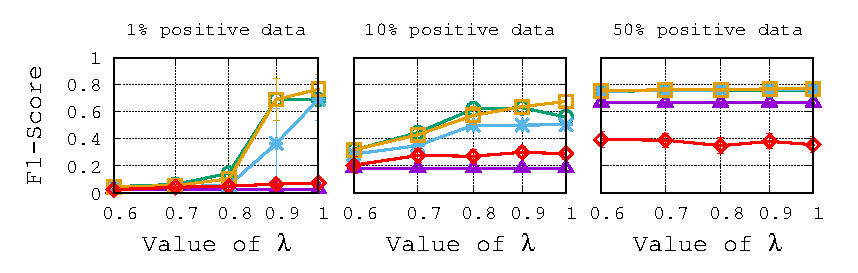
\includegraphics[width=14cm]{f1_performance_posrate_Data_150}}\par\end{centering}
\caption{Clustering algorithm performance vs. varying relevance noise ($\lambda$) for \#data=150.}
\label{fig:F1_vs_Lambda}
\end{figure}




%\subfour{Varying rate of positive data:} Here we aim to understand how the different F1-Score optimization algorithms perform as we vary the proportion of positively labeled ground truth data.
%Figure \ref{fig:F1_vs_Pos_Twitter} shows the results of this analysis while fixing the size of the data to 150 and $\lambda\in \{0.6,0.9\}$, and varying the rate of positive data in $[0.5\%,50\%]$.


%\begin{figure}[H]
%\begin{centering}
%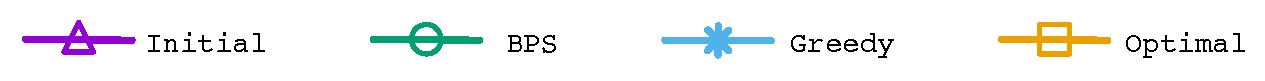
\includegraphics[width=8.5cm]{imgs/legend1}
%\par\end{centering}
%\begin{centering}
%{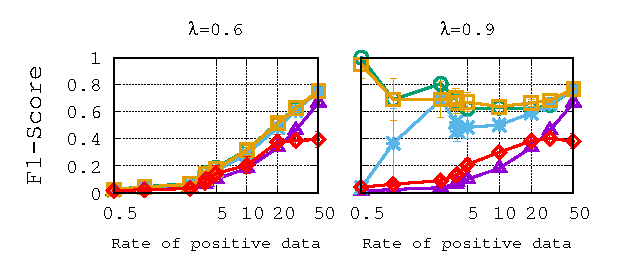
\includegraphics[width=7.75cm]{imgs/Twitter_results/f1_performance_Data_150}}
%\par\end{centering}
%\caption{Performance with \#data=150.}
%\label{fig:F1_vs_Pos_Twitter}
%\end{figure}

%Briefly, we note again that all curves of the same algorithm with the same parameters have the same shape across the different datasets.

%Briefly, we observe that the problem becomes easier as the number of positive examples increases as well as the value of $\lambda$ increases (i.e., noise decreases). 
%This is explained by the fact that a high rate of positive examples allows the algorithms to be able to select a subset of elements with a large number of positive examples thus maximizing F1-Score. However, a low value of $\lambda$ tends to lead the algorithms to select all content (close to Initial set) due to the level of noise, while a high value of $\lambda$ tends to lead the algorithms to select the actual positive examples and thus maximize F1-Score. This is shown through the increasing separation of all curves from the Initial curve as $\lambda$ increases.  $k$-means does not outperform Initial.

%(Fig 78a,d = \#data=150, lambda=0.6/0.9 X 3 domains).  Add lambda=1 if fits.








%\subfour{F1-Score vs. EF1-Score:} This analysis aims to answer the following question: \textquotedblleft \textit{Under what conditions is EF1 is a good surrogate for F1?}\textquotedblright{}. The results of this analysis are shown in Figure \ref{fig:F1_vs_EF1_Enron} using a set of four scatter plots.
%We show a comparison of the results obtained when optimizing the real F-Score vs. those obtained when optimizing expected F1-Score with different values for $\lambda$.
%To provide more clarity, the line $y = x$ is included to convey whether the optimization of a particular set gave the same F1-Score using the different optimization strategies or not. A point above the line corresponds to a set for which the optimization with EF1-Score gave a higher F1-Score, while a point below the line refers to a set for which the optimization with EF1-Score  hurts the F1-Score. We also include the plot of the function that fits the data points to show how far is the expected F1-Score with respect to the real F1-Score. In addition, we provide a global Root Mean Square Error (RMSE) value to get an overview of the approximation.

%Briefly, it is clear that for high values of $\lambda$ (e.g., 0.9), the optimization with EF1 gives a good approximation of the real F1-Score, with RMSE=0.01 for $\lambda=0.9$. For a lower $\lambda=0.8$ and $\lambda=0.6$ we do observe significantly more noise (as expected), but we also note from the assymetry that EF1 effectively lower bounds the true F1 score indicating the desirable optimization property that high EF1 implies high F1-score.
%, the RMSE is respectively multiplied by 3 and 8, indicating that for high noise, the approximation may completely be reduced to a random value. Hence, we conclude that for a classifier with a high accuracy (say 80-90\%), the expected F1-Score is a good approximation for the real F1-Score.

%\begin{figure}[H]
%\begin{centering}
%\par\end{centering}
%\begin{centering}
%{\includegraphics[width=8cm]{imgs/scatter_plot2_EF1\ly%xdot vs\lyxdot F1}}
%\par\end{centering}
%\caption{Scatter plot showing EF1-Score vs. F1-Score.}
%\label{fig:F1_vs_EF1_Enron}
%\end{figure}


%\begin{figure}[H]
%\begin{centering}
%\par\end{centering}
%\begin{centering}
%\includegraphics[width=9cm]{imgs/boxplot2_EF1\lyxdot vs\lyxdot F1}
%\par\end{centering}
%\caption{EF1-Score vs. F1-Score.}
%\label{fig:Time_vs_Pos_Reddit}
%\end{figure}




%\subfour{Analysis of the multiple filter selection wrapper strategy:} Figure~\ref{fig:FilterWrapperStrategy} shows how many filters it takes (x-axis) to reduce the number of non-filtered emails above the score threshold of $S(j)=0.6$ to zero (y-axis).  A faster reduction to zero indicates better coverage with fewer filters.  We observe the following: (1) for higher relevance noise, fewer filters are needed since all methods tend to return most elements in the first filter, (2) BPS tends to return the highest number of filters, followed by the Optimal MILP method, then the Greedy method, and (3) all methods tend to quickly return filters (at most 5 filters) that cover the relevant elements with a probability score higher than 0.6.



%\begin{figure}[H]
%\begin{centering}
%
\includegraphics[width=8.5cm]{imgs/legend2}
%\par\end{centering}
%\begin{centering}
%\subfigure[$\lambda=0.8$.]{\includegraphics[height=2.24cm]{imgs/wrapper/wrapper_posrate_30\lyxdot 0_lambda_0\lyxdot 8_rate_data_150}}
%\subfigure[$\lambda=0.9$.]{\includegraphics[height=2.24cm]{imgs/wrapper/wrapper_posrate_30\lyxdot 0_lambda_0\lyxdot 9_rate_data_150}}
%\subfigure[$\lambda=1.0$.]{\includegraphics[height=2.24cm]{imgs/wrapper/wrapper_posrate_30\lyxdot 0_lambda_1\lyxdot 0_rate_data_150}}
%\par\end{centering}
%\caption{Effect of the filter wrapper strategy on the Twitter dataset with 30\% of positive data and \#data=150.}
%\label{fig:FilterWrapperStrategy}
%\end{figure}



%\subsection{Computational time complexity analysis}
%We now report experimental results under the previous settings in terms of time complexity for  scalability analysis.


%\subfour{Time  vs. \#data:} A critical question for scalability is how time complexity of cluster optimization scales vs. the amount of data.  Figure \ref{fig:Time_vs_Data} reports the results of this analysis on the three datasets while fixing the rate of positive data to 2\% and $\lambda=0.9$, and varying the size of the data.
%Naturally, the problem becomes harder as the size of the data increases.  
%We also observe that Enron has highest time complexity followed by the Reddit dataset, and then the Twitter dataset. This is certainly due to the fact that the size of the text associated with each entity in each dataset is different, ranging from dozens of thousands of characters for emails in Enron to 144 characters for tweets in Twitter. Hence, more words increase the time complexity. 
%Overall, we critically notice that the BPS algorithm tends to have a lower time complexity than the greedy algorithm making it the most scalable of those compared.

%More complex case for \%malicious.  High noise makes for a hard problem, but increasing \%malicious just causes it to select everything (easy).  Low noise, not much to select for low \%mal, but have to work hard to select the right 50\% for high \%mal.  For moderate noise see both effects! 


%\subsection{[Last] Computational time performance (Fig 107d, 117f, 130a,c,e.)  For all 3 domains if space, but not necessary.}

%\begin{figure}
%\begin{centering}
%
\includegraphics[width=8.5cm]{imgs/legend2}
%\par\end{centering}
%\begin{centering}
%{\includegraphics[width=6.0cm]{imgs/Twitter_results/time_posrate_2\lyxdot 0_0\lyxdot 9}}
%\par\end{centering}
%\caption{Time complexity: 2\% positive data and  $\lambda=0.9$.}
%\label{fig:Time_vs_Data}
%\end{figure}



%\subfour{Time vs. $\lambda$:}  Another question is how noise levels in relevance prediction affect the time complexity of cluster optimization.  The results of this analysis are shown in Figure \ref{fig:Time_vs_Lambda} while fixing the rate of positive data in  \{3\%,20\%,30\%\} and the size of the data to 150, and varying the amount of noise of the classifier $\lambda \in [0.6,1.0]$.

%In brief, we first notice that clearly, for low rate of positive data (3\%) and with $\lambda=0.6$, the optimization algorithm has a high time complexity (up to 30 second to find the optimal solution). Hence, the optimal solution is clearly not scalable. Moreover, we observe that this time complexity reduces as the value of $\lambda$ increases. We explain that by the fact that the algorithms need to make a large number of iterations to find the best solution with high noise (low $\lambda$). \textcolor{red}{However, we observe an inverse effect for a high rate of positive data. Indeed, with 50\% of positive data the highest is the value of $\lambda$ the highest is the time complexity due to the fact that the optimal solution is hard to compute. For moderate rate of positive data we observe a stable time complexity as we vary  $\lambda$.}



%\begin{figure}
%\begin{centering}
%
\includegraphics[width=8.5cm]{imgs/legend2}
%\par\end{centering}
%\begin{centering}
%{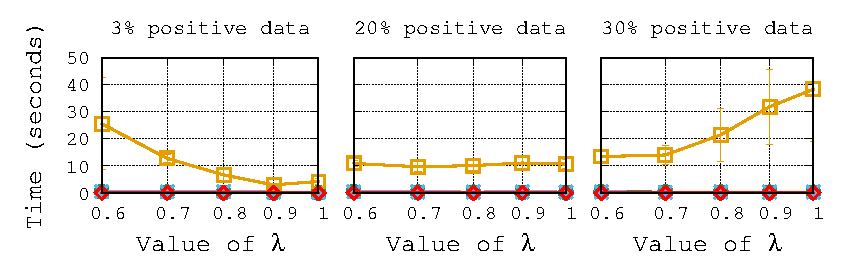
\includegraphics[width=8.75cm]{imgs/Twitter_results/time_posrate_Data_150}}
%\par\end{centering}
%\caption{Time complexity:\#data = 150.}
%\label{fig:Time_vs_Lambda}
%\end{figure}

%\subfour{Time vs. rate of positive data:} Finally we ask how changes in the proportion of positive data affect the time complexity of filter optimization.  Figure \ref{fig:Time_vs_Pos_Twitter} shows the results of this analysis while fixing the  the size of the data to 150 and $\lambda\in \{0.6,0.8,1.0\}$, and varying the rate of positive data in $[0.5,50]$.




%\begin{figure}[H]
%\begin{centering}
%
\includegraphics[width=8.5cm]{imgs/legend2}
%\par\end{centering}
%\begin{centering}
%{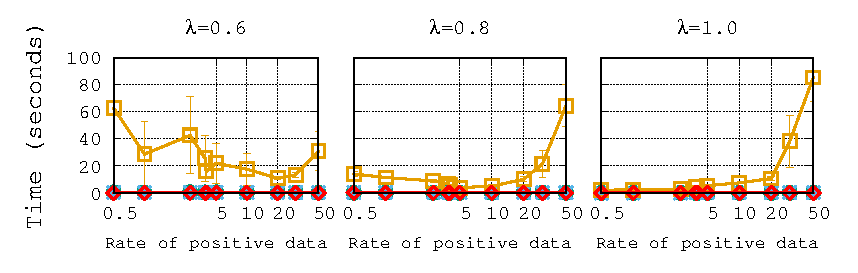
\includegraphics[width=8.75cm]{imgs/Twitter_results/time_Data_150}}
%\par\end{centering}
%\caption{Time complexity on Twitter with \#data=150.}
%\label{fig:Time_vs_Pos_Twitter}
%\end{figure}



%Here again we observe that the results are consistent across the different datasets. 
%At first glance, we observe that high noise (low $\lambda$) makes a hard problem for the optimization algorithm, but increasing the rate of positive examples causes it to select everything (making the problem easier).  For low noise (high $\lambda$), only a few elements are selected for a low rate of positive data, but the optimization algorithm has to work hard to select the right 50\% for high rate of positive data.  For moderate noise we observe both effects.



%At first glance, we observe that for small values of $\lambda$ the time complexity for the optimization algorithm tends to increase while decreasing rate of positive data. However, for high values of $\lambda$ the time complexity for the optimization algorithm tends to increase while increasing  the rate of positive data. 





%In both cases, we explain that by the fact that This is probably because the optimization algorithm fails in discrimination positive from negative examples.


%\subsection{Summary of findings}
In conclusion, the evaluations have shown that the \textcolor{red}{{\bf RadiCAl-Greedy}} and \textcolor{red}{{\bf RadiCAl-BPS}} algorithms are a good approximation of the Optimal MILP formulation (\textcolor{red}{{\bf RadiCAl-MILP}}) and may outperform the \textcolor{red}{{\bf RadiCAl-MILP}} in high noise settings --- especially the \textcolor{red}{{\bf RadiCAl-BPS}} approach which tends to overfit less to noise.  While this offline evaluation methodology allows direct head-to-head comparison of clustering algorithm properties and demonstrates potential advantages of \textcolor{red}{{\bf RadiCAl-BPS}}, what we need to experiment with next is whether \textcolor{red}{{\bf RadiCAl-BPS}} and our relevance-driven clustering approach enhance actual user performance in an online end-to-end visual search task.
%can be easily applied in very large scales, without any user intervention, hence it can be efficiently used for tuning the system parameters, and to efficiently examine and compare with other clustering baselines. 
% NOTE from Scott: I removed the following because it's hard to say that our data curation, ground truth knowledge, and handling of relevance scores in Section 7 does not introduce additional complications over the offline method.  I don't think the reviewer was asking explicitly for a criticism of the offline method, so I think we can skip this.
%However, due to the limitations of the evaluation methodology related to (1) assuming knowing the ground truth and (2) incorporating random noise sampled from a uniform distribution, conclusions based on the evaluation should be augmented with  complementary evaluation methods such as the user study we perform next.

%We have also shown that the BPS performs well in terms of objective optimization and is most efficient for scaling to large datasets.} 
%Finally, we have demonstrated that the expected F1-Score metric is a good surrogate of the F1-Score metric.}
%specifically when using an accurate classifier (roughly 80-90\% accuracy). 




\section{Study 2: User study}
\label{sec:UserStudy}
To complement and validate the results of the offline evaluation, we ran a user study with 24 subjects to measure the performance and preference of users with different clustering algorithms for a visual search interface.  In the following, we first briefly describe the way we estimate the relevance probability of each tweet in the visual search interface of the user study, then we describe the full user study methodology, and finally we end with an analysis of user performance.



\subsection{Relevance Scoring}
The underlying search and relevance scoring tool we developed for this user study was built on top of the Lucene IR System\footnote{http://lucene.apache.org/}.
% Not clear to me what "conventional" means -- not critical, I think.  -Scott
%, which adopts a conventional IR approach for both querying and retrieving tweets. 
As shown in Figure~\ref{fig:ScreenShot}, the interface allows users to enter a multi-term search query $q$, which retrieves the set $E_q$ of top-ranked 1,000 tweets according to their probability of relevance. 
As we previously defined in our relevance-driven clustering approach, terms (a.k.a. keywords) can be included/excluded by the clustering algorithm during the cluster extraction process.  However, in this user study, terms also enable us to derive the probability of relevance of a tweet to the user query.  Specifically, we used the standard information retrieval Language Model relevance scoring method as defined in~\cite{Zhai2001} for estimating the relevance score of a tweet $j$ w.r.t. a user query $q$ as follows: 
\begin{equation}
  S_q(j) = p(q|j) = \prod_{i=1}^n p(q_i|j) \,.
\end{equation}
Here, $p(q_i|j)$ is a unigram language model based on the tweet content $j$ calculated according to a Bayesian smoothing language model using Dirichlet priors as described in~\cite{Zhai2001} (Section~3). The relevance score provides the probability of relevance for each tweet that is subsequently used to compute and optimize the \textit{expected} F1-Score cluster extraction for our relevance-driven clustering.


\begin{figure}[t]
\begin{centering}
{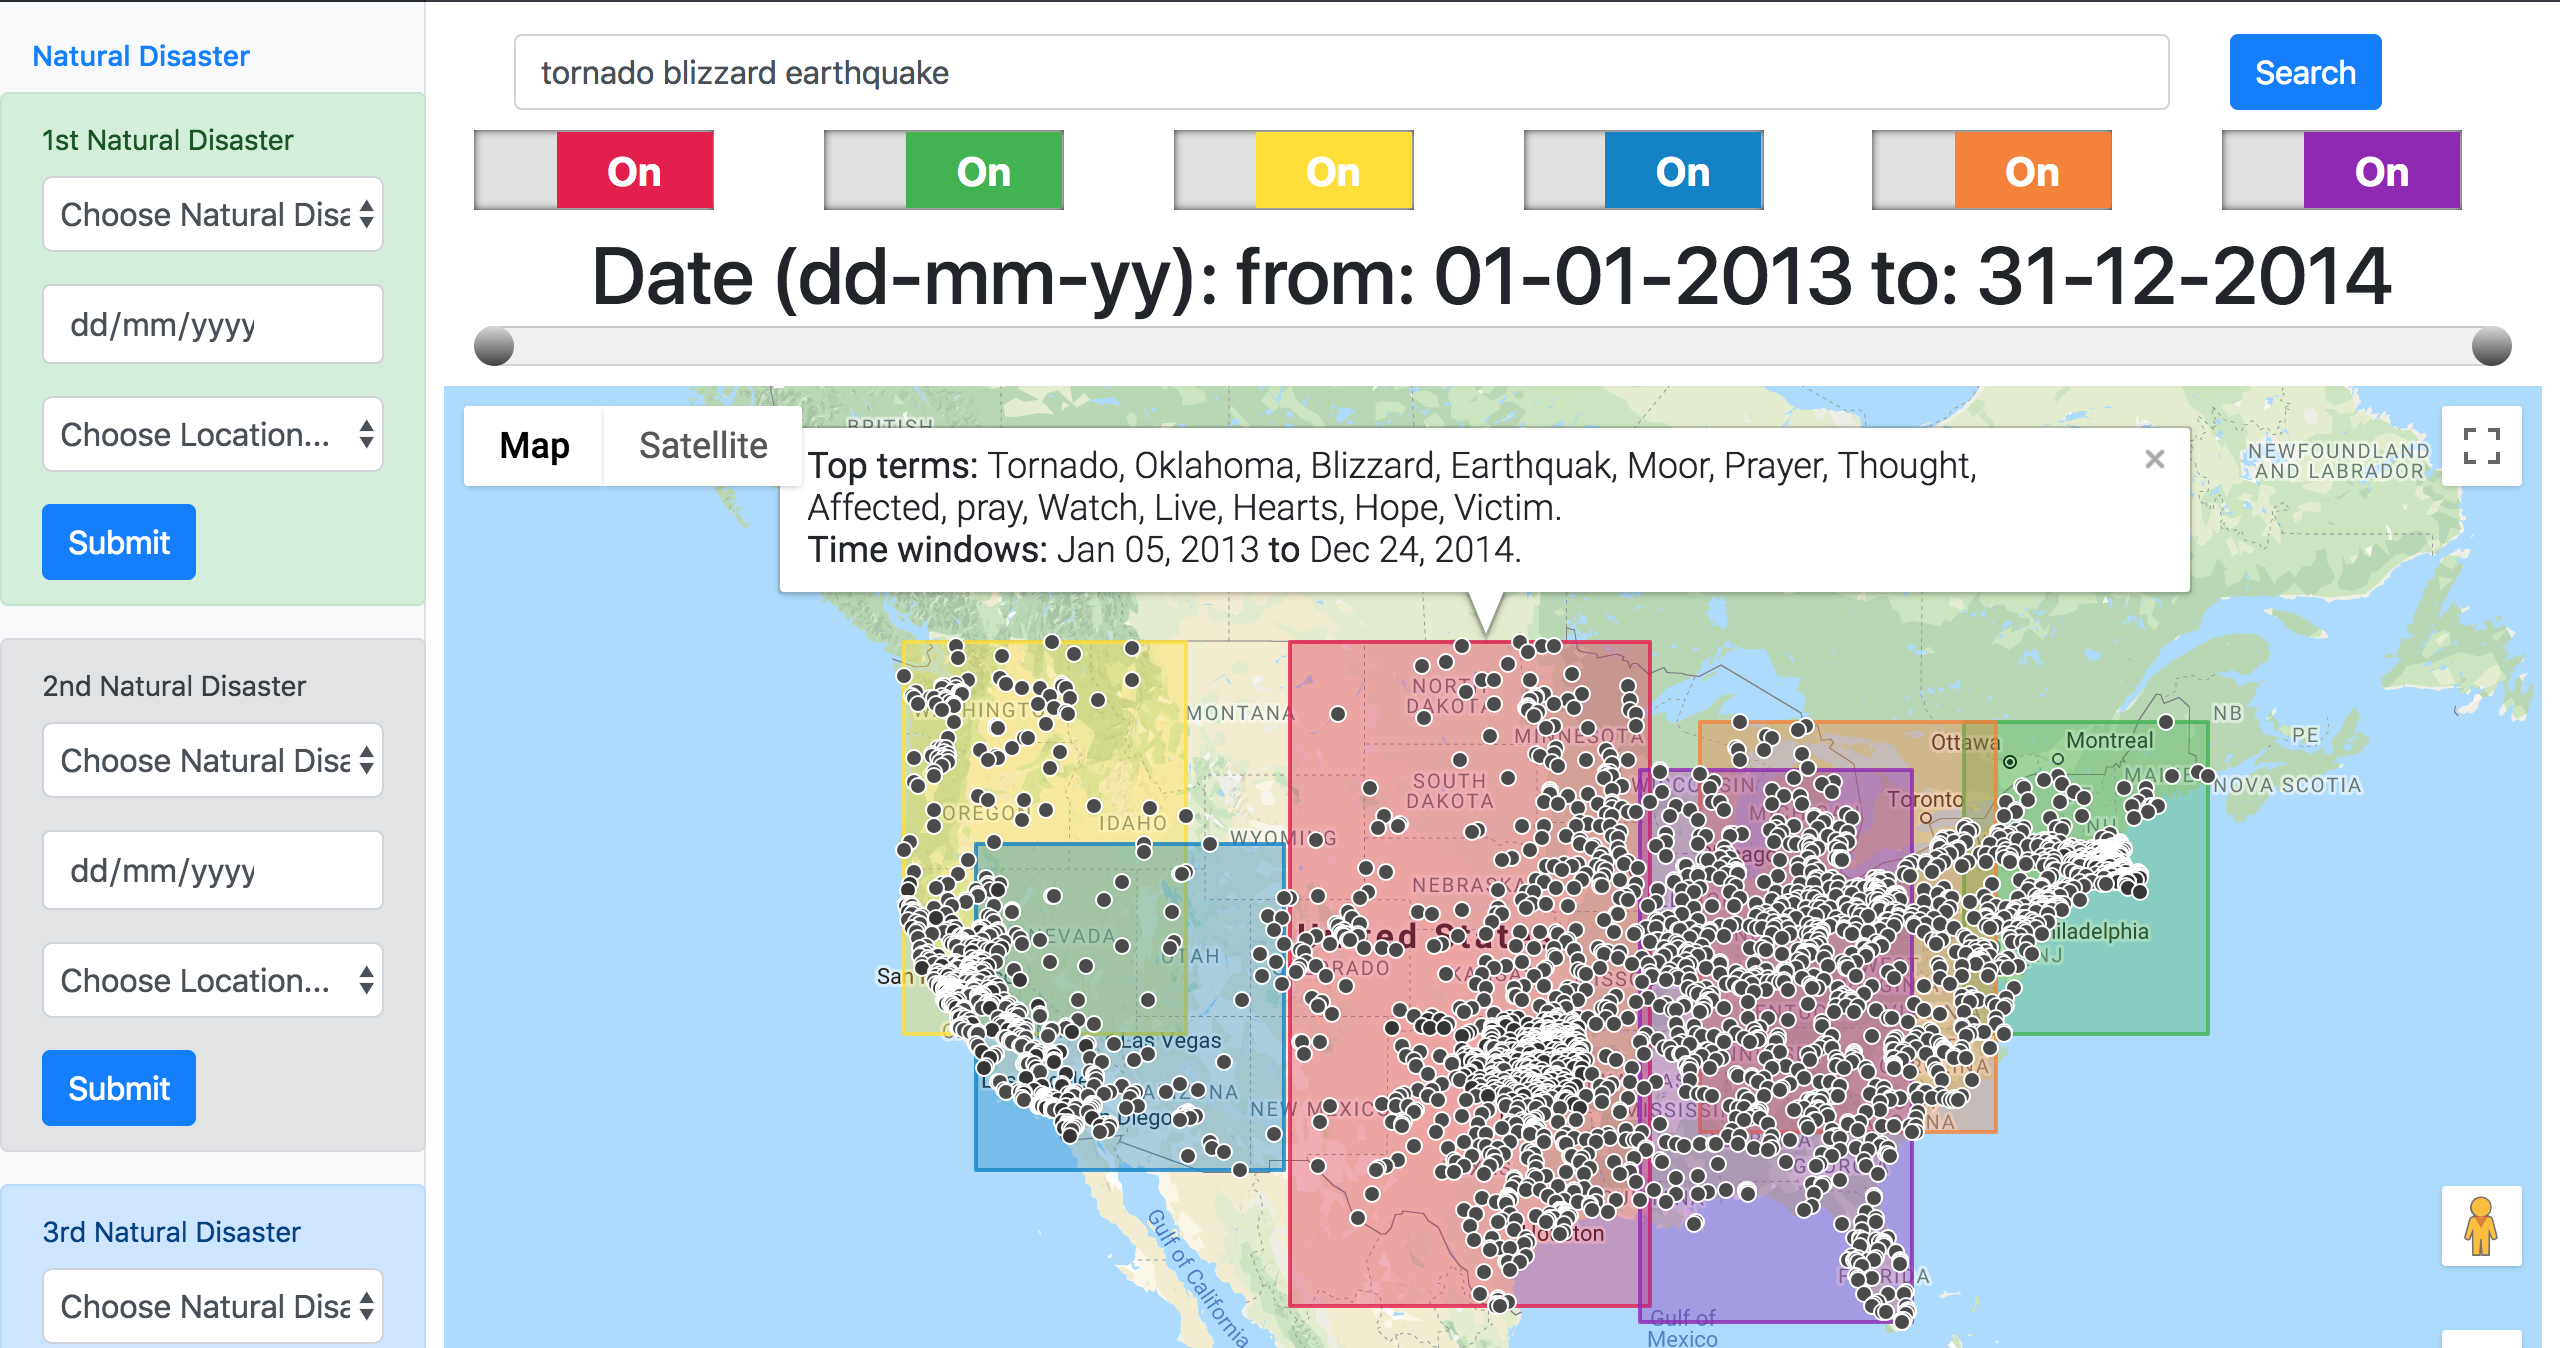
\includegraphics[width=16cm]{kmeans}}
\par\end{centering}
\caption{Clustering-based visual search interface. The results of the query ``tornado, blizzard, earthquake''  are shown using clusters of $K$-means. The top bar provides both a search box as well as buttons to explicitly hide or show clusters in the map display that allow the user to navigate and analyze clusters even when they overlap (e.g., as occurs with the yellow and blue clusters).  The left sidebar is used to provide answers in our experimental user study evaluated in this section.}
\label{fig:ScreenShot}
\end{figure}


\subsection{Research Hypotheses and Evaluation Methodology}
\label{sec:methodology}


The main goal of this user study was to comparatively evaluate human performance and visual search interface preference using three different search interfaces for identifying facts about natural disaster data in the previously described Twitter dataset.  The primary two hypotheses that we aimed to evaluate with human subjects were the following: ({\bf H1}) a clustering-based interface leads to better search performance and is more preferred than a non-clustering {\bf Baseline} interface, and ({\bf H2}) the relevance- and interface-driven clustering of \textcolor{red}{{\bf RadiCAl-BPS}} leads to better search performance and is more preferred by users than {\bf $\mathbf{K}$-means}.  

Over a sequence of three trials, each using a randomized (non-overlapping) selection of three natural disasters chosen from Table~\ref{tbl:events}, each of our users was asked to use one of the following three different search approaches (with the order of the three search approaches randomized for the three trials of each user):
\begin{enumerate}%[leftmargin=*]
\item A {\bf Baseline} multiple filter search method which displays {\bf all results that match the query}.  An example of the map portion of the display is shown in Figure~\ref{Fig:GlobalDisplay} with relevance shown as a gray-level shading.  While pan and zoom modulate the spatial filter, a time range adjustment filter is provided in addition to a keyword search filter to control inclusion/exclusion of content with specific terms.
\item The {\bf $\mathbf{K}$-means} algorithm discussed previously in the offline evaluation (using $X$-means to automatically identify the best $K$), which displays the {\bf largest 6  clusters for results matching a query} (an example is shown in Figure~\ref{fig:ScreenShot}).
\item The \textcolor{red}{{\bf RadiCAl-BPS}} algorithm we proposed for relevance-driven clustering that substantially outperformed the {\bf Greedy} approach in the offline experimentation. To match the presentation of {\bf $\mathbf{K}$-means}, \textcolor{red}{{\bf RadiCAl-BPS}}  displays the {\bf top 6 EF1-scoring clusters for results matching a query} (an example with 3 clusters is shown in Figure~\ref{Fig:BPS_FilteredDisplay}).
\end{enumerate}
Overall, we believe that the {\bf $\mathbf{K}$-means} and multiple filter {\bf Baseline} represent ideal methods for comparison to \textcolor{red}{{\bf RadiCAl-BPS}} since the first is arguably the most commonly used clustering method used in practice and the latter represents the manually-driven multiple filter search approach that \textcolor{red}{{\bf RadiCAl-BPS}} is attempting to automate through optimized relevance-based extraction of clusters defined by filter criteria.
Though use of the {\bf Baseline} method would be visually apparent to users, users were not aware of which clustering algorithm they were using in a trial that used either {\bf $\mathbf{K}$-means} or \textcolor{red}{{\bf RadiCAl-BPS}} clustering.
%trained to use the different search algorithms to find three different natural disasters.% using both a baseline interface showing all results as well as a clustering interface.

 
For each search approach, the interface allows users to enter a multi-term search query.
In the {\bf Baseline} search approach, these tweets are displayed on a Google Maps display used to browse the results.
The tweets that match a query were represented using circles with a grayscale color range corresponding to the probability of relevance -- light gray circles represented low probability relevance tweets, and dark gray circles represented high probability relevance tweets.
The user was able to interact with the map by panning and zooming and also by clicking on tweets to see their content.
The clustering search approaches ({\bf $\mathbf{K}$-means} and \textcolor{red}{{\bf RadiCAl-BPS}}) were identical to the
{\bf Baseline} search approach, except that instead of showing all matching results, they showed six clickable clusters of results as illustrated in Figure~\ref{fig:ScreenShot} (clicking a cluster displays a summary view and clicking a tweet in the cluster displays the specific tweet content).
In all search approaches, the user could use a time slider bar to restrict the results to tweets matching the query in a specific time window. 
%Once each user had familiarized themselves with the interface, they were asked to find three other natural disasters using a different display algorithm (baseline, $k$-means, EF1 relevance-driven clustering using the BPS greedy algorithm) for each of three trials containing three natural disasters each. 

\textcolor{red}{
Designing an Interactive IR evaluation approach is a challenging task for successfully evaluating exploratory search interfaces. This field has been widely explored and many suggestions have been provided for constructing simulated scenarios and tasks in order to engage participants in the search in a way that is as close as possible to actual information searching and IR processes~\cite{borlund2003iir,Kelly2009}.
Specifically, before starting the experiment, basic instructions were given to each participant among which not make a break, not to use their phone, and not to use social media such that to still focused on the task and perform a fair evaluation. We have collected basic information related to each participant including the English level, the education degree and the extent to which they are aware of natural disasters. The purpose of that entrance survey was to make sure that there is no bias among the participants.
Before starting the formal experiment, each participant was shown a training video describing the visual search interface, how to use it and how to interact with the clusters.  Then, each user was tested on his ability to find each of three natural disasters from Table~\ref{tbl:events} 
%(disjoint from the disasters used in the three experimental trials) 
using both the {\bf Baseline} non-clustering interface as well as the {\bf $\mathbf{K}$-means} clustering interface in two training trials. 
It was important to make sure that each user understood the global task before starting the formal experiment, thus the need for a training phase.
In each of the two training trials and the three experimental trials, the user was asked to enter information related to each natural disaster they identified, including the type of the natural disaster (e.g., earthquake, hurricane, flood, etc.) selected from a drop-down list, its location (US state) selected from a drop-down list, and the date (day) on which they think the disaster first occurred selected from a calendar chooser; the area where this information is entered can be seen on the left-hand bar in Figure~\ref{fig:ScreenShot}.}
It is important to reiterate that \emph{none} of the three experimental trials reused data from a previous trial.
%Once users chose correctly in the two training trials, they were allowed to proceed to the three experimental trials.
%by correctly identifying the time (day), location (US state), and type (earthquake, hurricane, etc.) of the natural disaster, 
A total of 24 users participated in the user study, for which the full experiment 
%two training and three experimental trials 
took on average 50 minutes per user.

We collected detailed interaction logs to record different behaviors and actions of the user. Moreover, each user was asked to answer NASA Task Load Index (NASA-TLX)~\cite{HART1988139} and System Usability Scale (SUS)~\cite{brooke1996sus} questionnaires after each trial. Finally, at the end of the experiment, each user was asked to fill out an exit survey, which included a preference ranking of the algorithms.

%The probability relevance score $S(j)$ of each tweet is an estimation of the conditional probability $p(q|t)$ that a tweet $t$ is relevant to the query $q$. To obtain this probability estimate, we used a language model scoring approach, which assumes that the individual terms $q_i$ of a query $q$ are ``generated'' by a probabilistic model based on the content of tweet $t$, thus directly estimating $p(q|t)$. 
%Also, for each user the sequence of algorithms to evaluate was presented differently, such that to cover all possible six combinations uniformly four times (24 users).  Here, we wish to indicate that the user had no indication of what algorithm was used each time, especially between the BPS and the $k$-means algorithms, which both present the results in a similar way using clusters (bounding boxes). 
%Finally, we highlight the fact that during we have set up the task such that it wasn't too easy nor too difficult for the user. 



% Figure \ref{fig:ScreenShot} shows the interface of the user study, with the results of the query ``tornado, blizzard, earthquake''  using $k$-means. The results of the same query with the baseline and the BPS algorithms are shown in Figure \ref{Fig:UseCase}. At first glance, we clearly observe that the clusters of the BPS algorithm are more focused and more contextualized than those of the $k$-means algorithm.  In the following, we analyze the main outcomes of this user study.



\begin{figure}[t]
\begin{centering}

\includegraphics[width=14cm]{legend3}
\par\end{centering}
\begin{centering}
{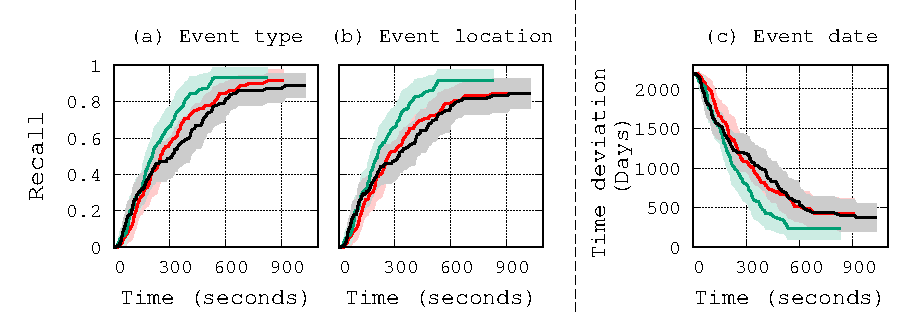
\includegraphics[width=16cm]{nd_recall}}
\par\end{centering}
\caption{The mean user performance and 95\% confidence intervals for each of the three search interfaces/algorithms are measured using cumulative recall for the type and location of the natural disasters and the absolute error for the first date of the natural disaster.  On average, users achieved higher recall and lower error faster using relevance-driven clustering (\textcolor{red}{{\bf RadiCAl-BPS}}) in comparison to $K$-means and the Baseline.}
\label{fig:UserSurveyRecall}
\end{figure}





%However, 
%\begin{figure*}[t]
%\begin{centering}
%
\includegraphics[width=7.5cm]{imgs/legend4}\\
%\subfigure[Natural disasters.] {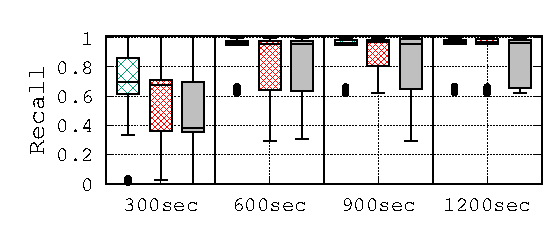
\includegraphics[width=5.7cm]{imgs/nd_recall_steps}}
%\subfigure[Locations of the natural disasters.] {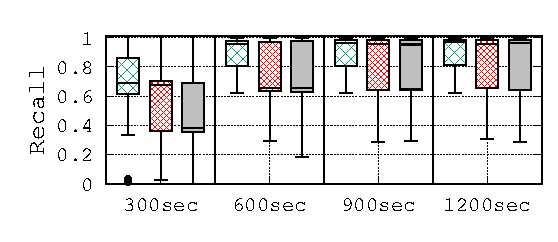
\includegraphics[width=5.7cm]{imgs/location_recall_steps}}
%\subfigure[Errors in the dates of the natural disasters.] {\includegraphics[width=5.7cm]{imgs/nd_time_deviation_recall_steps}}
%\par\end{centering}
%\caption{Performance of the algorithms measured at different elapsed times for each trial.}
%\label{fig:UserSurveyRecallStage}
%\end{figure*}



\subsection{Quantitative performance analysis}
\label{sec:quant_performance_analysis}

The performance of the users for each algorithm was measured using cumulative recall for the type and location of the natural disasters in each trial.  Since there were three distinct natural disasters per trial,  perfect recall would require getting all three natural disaster types or locations correct.  Mean performance across all users with 95\% confidence intervals for cumulative recall of disaster type and location are respectively shown in Figures~\ref{fig:UserSurveyRecall}(a) and~\ref{fig:UserSurveyRecall}(b).  Users also had to enter their estimated starting date of each natural disaster, which we measure by absolute error assuming the maximum error for natural disasters that have not been submitted yet.  The mean performance of time estimation error across all users with 95\% confidence intervals is reported in Figure~\ref{fig:UserSurveyRecall}(c).  %Moreover, in Figure~\ref{fig:UserSurveyRecallStage} we report the progression of these metrics for each algorithm using boxplots at different elapsed times into the experiment -- at 300, 600, 900 and 1200 seconds.

%While the %results of Figure~\ref{fig:UserSurveyRecall} 
%number of users in our study and the 95\% confidence intervals 
%do not permit strong claims of statistical significance
Regarding the quantitative portion of hypotheses H1 and H2, there are very consistent user performance trends that emerge after 150 seconds into the trial in Figure~\ref{fig:UserSurveyRecall}.  In the first 150 seconds, it would appear that all users were adjusting to the given task and some users were able to identify some of the most salient natural disasters that would have been obvious regardless of the interface type.  It seems that it is beyond this initial stage when users are searching for the remaining less salient natural disasters when the interface helps differentiate human performance.
%(i) 
Specifically, after 150 seconds in Figure~\ref{fig:UserSurveyRecall},  \emph{we observe the general trend that, on average, users achieved higher task recall and lower error faster} when using the \textcolor{red}{{\bf RadiCAl-BPS}} algorithm for clustering in comparison to {\bf $\mathbf{K}$-means} and the {\bf Baseline}.  
% The performance obtained for this user study confirms clearly the results obtained in the off-line evaluation since the BPS algorithm outperforms $k$-means and the baseline in identifying the natural disasters, their locations, and their dates.
%(ii) In general, the clustering approach is clearly useful for this kind of task as both BPS and $k$-means outperformed the baseline that show all matching elements. 
%(iii) Clearly, the BPS algorithm required much fewer efforts and time to complete the task than for $k$-means and the baseline and that to reach a bit higher level of recall.
%(iv) 
%Further considering the performance progression shown in Figure~\ref{fig:UserSurveyRecallStage}
Furthermore, we clearly notice that with the \textcolor{red}{{\bf RadiCAl-BPS}} algorithm, participants were able to achieve a \emph{higher average ``asymptotic'' performance at an earlier stage of the experiment} than using the two other search algorithms.  Such results quantitatively support both of our experimental hypotheses H1 and H2 from Section~\ref{sec:methodology} that motivated our study.

% As a conclusion for this evaluation, we notice that there is a similar outcome between the two evaluation methods -- the offline evaluation and the user study. Both evaluations confirm that the BPS algorithm
% the significant contribution of the BPS algorithm for this specific relevance-driven clustering task. Even though the off-line evaluation showed that $k$-means is inappropriate for this task, the performance obtained in this user study showed that it is effective to some extent. 




\begin{figure}[t!]
\begin{centering}

\includegraphics[width=14cm]{legend4}\\
\subfloat[Subscales rating. %``0'' means the user thinks that the workload for the considered dimension was ``Low'' and ``20'' means it was ``High''.
] {\hspace{0.4cm} 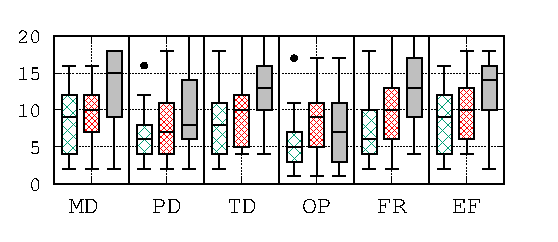
\includegraphics[width=9.0cm]{NASA_TLX}}
\subfloat[Overall rating.] {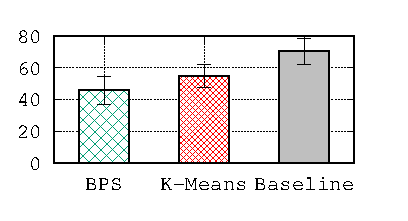
\includegraphics[width=7.5cm]{NASA_TLX_AVERAGE}}
\par\end{centering}
\caption{NASA Task Load Index (MD: Mental Demand, PD: Physical Demand, TD: Temporal Demand, OP: Own Performance, FR: Frustration, EF: Effort).  Higher numbers indicate higher perceived workload.}
\label{fig:NASA}
\end{figure}

\subsection{Survey analysis}
\label{sec:surveys}

With the previous quantitative measures of user performance indicating the advantage of relevance-driven clustering, we next proceed to evaluate the users' own opinions of each interface/algorithm as collected in the user surveys discussed in the methodology.  During the user study, each participant answered 7 different questionnaires -- a NASA Task Load Index (NASA-TLX)~\cite{HART1988139} and a System Usability Scale (SUS)~\cite{brooke1996sus} questionnaire after using each algorithm, plus a final questionnaire. We report key results below.




\subsubsection{NASA-TLX analysis}

The NASA-TLX questionnaire rates perceived workload in order to assess a task, system effectiveness or other aspects of performance.
The questionnaire includes questions on mental demand (MD), physical demand (PD), temporal demand (TD), performance (OP), frustration (FR), and effort (EF). NASA-TLX items are rated on a 20-point scale (1 = low workload, 20 = high workload, except for OP where 1 = perfect and 20 = failure).
Overall, we hypothesize that the three most important factors for this visual search task are temporal demand (reduced time to complete the search task owing to better clusters), mental demand (the ability to focus analysis at the cluster level of abstraction as opposed to the tweet level), and effort (reduced effort to analyze clusters due to clear keyword summaries).  We conjecture that all of these task load reductions would follow from the increased coherence of the \textcolor{red}{{\bf RadiCAl-BPS}} relevance-driven cluster extraction compared to unsupervised {\bf $\mathbf{K}$-means} clustering and the lack of any automatic clustering in the {\bf Baseline}.

We show the NASA-TLX results obtained (a) for each subscale and (b) for the overall ratings in Figure~\ref{fig:NASA}.
Briefly, the mean overall NASA-TLX rating was $45.91\pm 8.86$ for \textcolor{red}{{\bf RadiCAl-BPS}}, $54.75\pm 7.41$ for {\bf $\mathbf{K}$-means}, and $70.41\pm 8.27$ for the {\bf Baseline}. 
A Friedman's test revealed an overall significant difference ($\chi^2(3)= 16.113, p=0.003 < 0.05$).
Holm-Bonferroni corrected post-hoc analyses with Wilcoxon signed-rank tests 
revealed that the difference between all pairs was significant ($p < 0.05$). %The difference between BPS and $k$-means wasn't significant. Moreover, there were no significant differences in the sub-scales between BPS and $k$-means.

We note that participants overall perceived the \textcolor{red}{{\bf RadiCAl-BPS}} algorithm to be more effective at helping them complete their search task in comparison to using {\bf $\mathbf{K}$-means} or the {\bf Baseline}.  
Considering each of the three aforementioned key factors (TD, MD, EF) deemed most relevant to the innovations of the \textcolor{red}{{\bf RadiCAl-BPS}} clustering algorithm, we remark that
\textcolor{red}{{\bf RadiCAl-BPS}} recorded the lowest median load on all three factors with {\bf $K$-means} somewhat behind in second place (indicating that some form of clustering still aided the visual search task) and the non-clustering {\bf Baseline} further afield with the highest loads.  
%\textcolor{red}{Considering each of these factors respectively for the best-performing BPS approach, we remark that users were able to (1) complete the task by issuing less queries leading to reduced temporal demand, (2) investigate clusters of tweets rather than individual tweets leading to reduced mental demand, and (3) obtain clear and coherent keywords summarizing each cluster, thus reducing the global effort required.}
Considering additional factors, global median rates of frustration and mental effort were around 10, which indicates that the task was neither too difficult, nor too easy.  Also, as the median rates of these two factors were lower for the two clustering methods than the baseline, we conclude that participants overall felt that clustering-based search provided a less frustrating and less mentally demanding interface for this task in comparison to the baseline, which displayed all search results. 
%
Finally, based on the task load rates where the \textcolor{red}{{\bf RadiCAl-BPS}} algorithm performed the best, it seems apparent that relevance-driven \textcolor{red}{{\bf RadiCAl-BPS}} clustering provided the most effective approach for carrying out this kind of spatio-temporal search task, which is supported by the overall rating of Figure~\ref{fig:NASA}(b).

% {\bf BPS} algorithm for clustering in comparison to {\bf $\mathbf{K}$-means} and the {\bf Baseline}.


\begin{figure}[t!]
\begin{centering}
% Note: legend not needed here.  -Scott
%
\includegraphics[width=10cm]{legend4}\\
{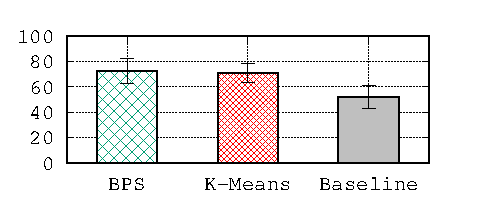
\includegraphics[width=9cm]{SUS_AVERAGE}}
\par\end{centering}
\caption{System Usability Scale overall rating.  Higher values indicate higher perceived usability.}
\label{fig:SUS}
\end{figure}

\subsubsection{SUS analysis}
The SUS questionnaire gives a global view of subjective assessments of usability. The questionnaire contains questions related to the global effectiveness, efficiency, and satisfaction. The SUS items are rated on a 5-point scale (0 = strong disagreement and 5 = strong agreement). In Figure~\ref{fig:SUS}, we show the results obtained over all SUS scores  with 95\% confidence interval. The mean SUS score was $72.39\pm 9.77$ for \textcolor{red}{{\bf RadiCAl-BPS}}, $70.83\pm 7.61$ for {\bf $\mathbf{K}$-means}, and $51.77\pm 9.07$ for the {\bf Baseline}. A Friedman's test revealed an overall significant difference ($\chi^2(3)= 9.053, p=0.010 < 0.05$).
Holm-Bonferroni corrected post hoc analyses with Wilcoxon signed-rank tests 
revealed that the difference between the two clustering methods and the baseline was significant ($p < 0.05$). The difference between \textcolor{red}{{\bf RadiCAl-BPS}} and {\bf $\mathbf{K}$-means} wasn't significant and hence we can only infer from the SUS survey that the users preferred the clustering interface (i.e., \textcolor{red}{{\bf RadiCAl-BPS}} and {\bf $\mathbf{K}$-means}) over the {\bf Baseline}.% display of all search results.





\begin{figure}[t!]
\begin{centering}

\includegraphics[width=12cm]{legend4}\\
{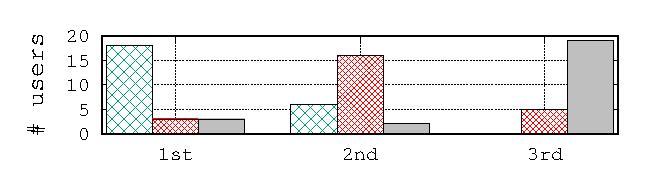
\includegraphics[width=14cm]{ranking}}
\par\end{centering}
\caption{Ranking of the algorithm preference by participants who voted by trial ID (not algorithm name).  The number of users who placed each algorithm at the specified ranking is shown.  Clearly, relevance-driven clustering (\textcolor{red}{{\bf RadiCAl-BPS}}) received the bulk of first place preference, K-means the bulk of second place preference, and Baseline the least preference at third place.}
\label{fig:UserSurveyRanking}
\end{figure}
\subsubsection{Final questionnaire analysis}
The final questionnaire that the users had to answer included questions on the advantages and disadvantages of each algorithm, plus a global ranking of the three algorithms. %Due to space limitations, we briefly summarize the top disadvantages of the BPS algorithm and advantages of the baseline method in Table~\ref{tbl:SurveyComments}.
%
% Preview source code for paragraph 0
%
%\begin{table}
%\caption{User survey comments.}
%\label{tbl:SurveyComments}
%\begin{centering}
%\begin{tabular}{|>{\centering}p{4cm}|>{\centering}p{4cm}|}
%\hline 
%\textbf{Disadvantages of BPS} & \textbf{Advantages of Baseline}\tabularnewline
%\hline 
%\hline 
%Clusters that have huge time-spend are most likely useless. & Simple, easy. Using %just the time sliders it was very easy to detect
%the disasters. \tabularnewline
%\hline 
%Does not show up all the data points.  & Using the timeslider, I found it more %useful than the filters. \tabularnewline
%\cline{1-1} 
%The interface takes more time to learn.  & \tabularnewline
%\hline 
%\end{tabular}
%\par\end{centering}
%\end{table}
%
The ranking of the algorithms provided by users is shown in Figure \ref{fig:UserSurveyRanking}. 
We note that 18 users out of 24 ranked \textcolor{red}{{\bf RadiCAl-BPS}} as being the best algorithm, and 19 users out of 24 ranked the {\bf Baseline} approach as being the least helpful for the task.  Hence there is strong evidence for user preference of \textcolor{red}{{\bf RadiCAl-BPS}} over {\bf $\mathbf{K}$-means} and for both \textcolor{red}{{\bf RadiCAl-BPS}} and {\bf $\mathbf{K}$-means} over the {\bf Baseline}.  In the free response survey section, several users also specifically reported the ease and precision provided by the trial with the \textcolor{red}{{\bf RadiCAl-BPS}} algorithm assigned, while no users indicated this for the trials with {\bf $\mathbf{K}$-means} or \textcolor{red}{{\bf RadiCAl-BPS}} assigned. % to complete this search task.

Combined with the quantitative performance analysis of Figure~\ref{fig:UserSurveyRecall} discussed in Section~\ref{sec:quant_performance_analysis} and the NASA-TLX workload and SUS usability survey results discussed in Section~\ref{sec:surveys}
that both corroborate these preference findings, we remark that all of the experimental evidence strongly supports hypotheses H1 and H2 from Section~\ref{sec:methodology} that motivated our user study. 
%However, we note that two users mentioned that they still prefer the baseline approach. 
%This is probably due to the fact that they are used to work with a conventional search approach, and that they couldn't digest this new search clustering paradigm. 


\section{Discussion}
\label{sec:Discussion}
\textcolor{red}{In this section, we discuss the main limitations of this research and the possible future work that we intend to investigate. }
%Overall, we aim for this work to bring a formal IR perspective to the important research area of AUIs while opening new research directions for the application of IR methodology.  As information
%retrieval has transformed our web experience, we believe there is
%a similar opportunity to transform the present nascent state of AUIs
%through optimization and information retrieval principles to make
%them more ubiquitous in our daily lives. 



%In this article, we have expanded on the information filtering paradigm of Belkin and Croft \citep{Belkin1992}, by  

  %We have also proposed a method for optimization of expected F1-score using a MILP approach that has critically allowed us to benchmark the greedy algorithms on moderate-sized datasets. 
\subsection{Summary of results}


\textcolor{red}{The aim of this research was to investigate relevance-driven clustering, which led to the development of novel optimization algorithms for expected F1-Score based on two different greedy strategies (\textcolor{red}{{\bf RadiCAl-Greedy}} and \textcolor{red}{{\bf RadiCAl-BPS}}). }
%
The offline evaluations we performed 
%on a Twitter dataset 
show that the binary partitioning search (\textcolor{red}{{\bf RadiCAl-BPS}}) algorithm we have proposed is relatively efficient, performs comparably to or exceeds $K$-means performance when the relevance signal is moderately reliable, and provides a good approximation of the \emph{optimal} MILP solution in small instances where comparison is possible.
%Somewhat surprisingly, we remark that greedy methods like BPS may even do better than exact expected F1-score optimization in high noise cases for relevance estimation due to the more restricted search space of BPS, which effectively prevents ``overfitting'' to this noise. 

The user study we carried out on 24 users confirmed the outcome of the offline evaluation and has demonstrated that our novel relevance-driven clustering based on  BPS (\textcolor{red}{{\bf RadiCAl-BPS}}) is highly effective for our search scenario.  Specifically we confirmed quantitatively that users achieved generally faster search task completion, higher recall, and lower error using relevance-driven clustering compared to $K$-means and a non-aggregation baseline.  Users also indicated that the \textcolor{red}{{\bf RadiCAl-BPS}} approach yielded lower perceived workload on the NASA-TLX survey and higher usability on the SUS survey.  And finally, to corroborate all of these findings, users ultimately indicated a strong first preference for the relevance and interface-driven clustering approach that comprises the novel contribution of this article.   All the algorithms described throughout this paper have been integrated into a tool called Visual Twitter Information Retrieval (Viz-TIR)~\cite{Bouadjenek2019}\footnote{\url{https://github.com/D3Mlab/viz-ir}}.

\subsection{Limitations}
\textcolor{red}{Even though the work described in this article have shown promising research perspectives, it suffers from multiple limitations at both the algorithmic and methodological levels. This includes:}
\begin{itemize}
\item \textcolor{red}{\emph{The limitation of a pure relevance-driven clustering approach.} The relevance-driven clustering approach we described in this paper has shown a very promising results presentation perspective by generating pure clusters around true events in terms of time, location and content. However, the algorithm may not generate clusters or alternatively generate only one big cluster in the case of a uniform distribution of the relevance in the search results. This issue should be addressed in future work by defining a new objective function to optimize that is also density-driven. }

\item \textcolor{red}{\emph{Adding more dimensions to the algorithm may not be trivial.} 
Although we mentioned previously that we don't limit this work to the three display attributes we used, incorporating more attributes may not be trivial and may involve some complex accommodations and adjustments in terms of programming. However, we believe that this should be feasible as long as it involves continuous or discrete cluster attributes. }

%\item Are there any theoretical implication w.r.t. to multi-objective optimization (Deb, 2014)? 

%\item Or any practical implications w.r.t. reranking in IR (Ghorab, 2012)?

\item \textcolor{red}{\emph{The expensiveness of user studies.}
Carrying out user studies is a time-consuming and expensive process since it involves human beings. Although we had a decent number of participants in our user study who were able to compare and assess three different algorithms, we believe that such a study and its conclusions should be reinforced with more participants as well as more algorithms to be compared.}

\item \textcolor{red}{\emph{The lack of context regarding natural disasters in the US for some participants.} Even though instructions and suggestions were given to the participants regarding the possible natural disasters to search, some participants mentioned the difficulty to come up with the right queries, mostly because of unfamiliarity with the US context.}

\end{itemize}

\subsection{Future Work}
Overall, we believe this work underscores the importance of relevance-driven clustering optimization methods specifically targeted for presentation in interactive visual search interfaces.  
However, there is still much more work to be done to fully explore the space of optimization objectives and algorithms for interactive visual search.  Interesting areas of future work include the following:
\begin{itemize}
%\item Consideration of the role of pseudo-relevance feedback~\cite{Manning2008} (Chapter 9) in a visual search and clustering setting.
\item \emph{Augmenting the relevance-focused F1-Score with additional cluster criteria to enhance word-level, spatial, and temporal coherence.}  While we argued and empirically demonstrated that our expected F1-Score cluster optimization objective does lead to coherently interpretable clusters, there is certainly the possibility to explore more complex objectives that may further enhance coherency for end users.  For example, research could explore novel application-specific objectives that take into account physical constraints of the display device as well as user cognitive constraints and preferences for cluster display that could be used to augment (or even replace) the existing F1-Score relevance-based objective.
\item \emph{Considering a ranking perspective of cluster relevance and optimization as opposed to a Boolean perspective.}  In this initial work, we did not want to address ranking aspects of visual clustering that might entail showing each result in a cluster as a different size since this would require consideration of psychovisual aspects of human information processing that are beyond the scope of the present article.  Nonetheless, such an extension is certainly possible in future work and would better leverage additional degrees of freedom in the search results display to distinguish results by their level of relevance.  A key challenge in such an extension would involve developing new optimization algorithms that could deal with the increased complexity of a ranking-style evaluation metric of cluster relevance.
\item \emph{Considering a topic modeling perspective in place of a clustering perspective.}  While clustering attempts to aggregate similar documents with the assumption that each document belongs to one cluster, topic modeling methods such as (probabilistic) LSA~\cite{deerwester1990,hofmann1999} or LDA~\cite{blei_lda} assume that a document is composed of multiple topics and try to estimate the degree or probability of relevance that a document has to each topic.  While topic modeling provides a more granular view of document content, such approaches pose a number of significant challenges for use with visual search interfaces.  Specifically, this would require highly effective spatio-temporal extensions of topic models, novel methods to visually display topics as opposed to clusters, extensions to topic modeling that explicitly consider relevance-based optimization criteria, and novel computational methods to effectively optimize within this extended framework.  Nonetheless, the benefits of a more granular topic modeling perspective may certainly motivate extensions of this work to \emph{relevance-driven topic modeling} for visual search interfaces.
\end{itemize}

\section{Conclusion}
\label{sec:Conclusions}
In this article, we have noted that while unsupervised clustering methods have often been used to aggregate data in visual search interfaces, approaches like $K$-means do not make effective use of query relevance signals during this aggregation task and do not necessarily optimize for purposes of visual presentation in the user interface.  To address these deficiencies, we introduced a cluster definition intended for spatial, temporal, and content coherence for visual presentation that does not require specification of complex distance metrics like $K$-means.  We have further introduced a novel formulation of relevance-driven clustering for visual search as an optimization problem given a probabilistic measure of relevance for search results.  We have motivated and derived expected F1-Score as an objective criteria for relevance-driven cluster optimization. % and we have experimentally demonstrated that the proposed expected F1-Score metric is a good surrogate of the ground truth F1-Score.
%
We introduced novel relevance-driven clustering approximate optimization algorithms for expected F1-Score based on two different greedy strategies (\textcolor{red}{{\bf RadiCAl-Greedy}} and \textcolor{red}{{\bf RadiCAl-BPS}}).



In sum, we hope that this article provides a first stepping stone to a wide range of exciting future work on the topic of relevance- and interface-driven clustering to help create the next generation of enhanced visual information retrieval systems.


% Important areas of future work include enhanced indexing strategies and scalability in filter selection algorithms along with the 
%Important areas of future work include consideration of the role of (pseudo-)relevance and other explicit or implicit feedback methods. % to create a tighter and more responsive user interaction loop.
%Furthermore, we should also consider novel application-specific objectives, e.g.,  in specific visualization frameworks. % or based on a ranking theory of results presentation (e.g., using size or color for visual ranking emphasis).  


% For future work, we are currently integrating these algorithms into our existing user interface of graph exploration and mining. We also plan to conduct a user study in the context of natural disasters discussed on twitter to analysis our algorithms and get a real insight of their accuracy. Finally, we plan to investigate new optimization metrics based on visual rendering.








\section*{Acknowledgements}

We thank two anonymous reviewers for their questions and comments, which helped to improve and clarify the article presentation and also provided numerous suggestions for our future work discussion. \textcolor{red}{All algorithms described in this paper, the material used,  as well as the tool we developed for the user study can be accessed here: \url{https://github.com/D3Mlab/viz-ir}.}

%\section*{References}

\bibliographystyle{unsrt}
\bibliography{biblio}

\appendix

%\newpage

\section{Optimal MILP Solutions for Benchmarking}
\label{sec:milpform}

In this Appendix, we outline the details of an exact Mixed Integer Linear Programming (MILP) optimization-based formulation to maximize EF1 that provides a benchmark for evaluating the two proposed relevance-driven algorithms (\textcolor{red}{{\bf RadiCAl-Greedy}} and \textcolor{red}{{\bf RadiCAl-BPS}}) proposed in Section~\ref{sec:Algorithms} intended to approximately optimize EF1.  %Given the trivial solution of optimizing the expected precision (singleton) and expected recall (the whole collection), we consider in the following only the optimization of EF1.  

\subsection{Fractional MILP Formulation} \hfill \\
Leveraging notation defined in Section~\ref{sec:Framework}, we begin by reformulating the EF1 objective to prepare for further optimization steps by replacing the global sum of scores of all information elements with a constant $C = \sum_{j=1}^m S_q(j)$:
\begin{equation}
\begin{aligned}
    \emph{$EF1$} &= \dfrac{2\times \sum_{j=1}^m S_q(j)I_q(j)}{\sum_{j=1}^m I_q(j) + \sum_{j=1}^m S_q(j)} = \dfrac{2 \times \sum_{j=1}^m S_q(j)I_q(j)}{\sum_{j=1}^m I_q(j) + C}
\end{aligned}
\end{equation}

In order to obtain the EF1-optimal cluster, we let binary variables $\emph{I\textsubscript{filter}}($j$) \in \{0, 1\}$ indicate whether an information element $j$ is selected in by each cluster parameter and constrain that to be selected in the Global cluster (i.e., $I_q(j)=1$), $j$ must be selected by all cluster parameters (i.e., a conjunction).  This leads to the following fractional MILP formulation with cluster parameter constraints to be defined later:
%intend to directly optimize the EF1 metric in terms of decision indication variables  for filter setting as follows:
% Don't use I(i)... confusing!  
%\begin{align}
%\max_{\textit{filter vars}} \;\;
%& \dfrac{\sum_{j=1}^m S(i)I(j)}{\sum_{j=1}^m I(j) + C} \nonumber \\
%& \textrm{subject to constraints between {\it filter vars} and $I(j)$}   
%\end{align}
\begin{equation}
\begin{aligned}
& \underset{I_{\mathit{cluster}}(j)}{\text{maximize}}
& & \dfrac{\sum_{j=1}^m S_q(j)I_q(j)}{\sum_{j=1}^m I_q(j) + C} \\
& s.t
& & I_q(j) = \bigwedge I_{\mathit{cluster}}(j) \\
\end{aligned} \label{eq:frac_milp}
\end{equation}

% Not necessary.  -Scott
%Note that our goal is to optimize the element set in terms of \emph{filters settings}. This means elements in the interface sharing the same property needs to be simultaneously added to the selected set. This is a unique property of our filter-based UI problem, which is different from the independent retrieval of each document in standard IR system.

\subsection{Transformation to a MILP} \hfill \\
While there are no direct solvers for fractional MILPs, we can transform~\eqref{eq:frac_milp} into a pure MILP form for which we have efficient and optimal solvers.  To do this, we use the Charnes-Cooper method \cite{Charnes1962} and Glover linearization method \cite{Glover1975} with big-M constraints, where auxiliary variables \emph{w(j)} and \emph{u} are  introduced\footnote{https://optimization.mccormick.northwestern.edu/index.php/Mixed-integer\_linear\_fractional\_programming\_(MILFP)}. Here, $w(j)$ is defined as $w(j)=I_q(j)\times u$ with $u$ defined as follows:
\begin{equation}
u = \dfrac{1}{\sum_{j=1}^m I_q(j) + C}
\end{equation}

Then, the EF1 optimization problem is able to be transformed into the following MILP problem:
\begin{equation}
\begin{aligned}
& \underset{w,u}{\text{maximize}}
& & \sum_{j=1}^m S_q(j)w(j) \\
& s.t
& & \sum_{j=1}^m w(j) + uC = 1 \\
& & & w(j) \leqslant u, \quad w(j) \leqslant M\times I_q(j)  \\
& & & w(j) \geqslant u - M\times [1-I_q(j)] \\
& & & u > 0,  \quad I_q(j) \in \{0, 1\}, \quad w(j) \geqslant 0 \label{eq:milp}
\end{aligned}
\end{equation}

\subsection{Additional MILP constraints for cluster definitions} \hfill \\
As our goal is to select information elements through cluster parameters that define spatial, temporal, and keyword coherence, we add three constraints to the above optimization to define each of these cluster criteria:
\begin{enumerate}
\item {\bf Time Selection Constraint:} a two-element tuple ($t_{start}$, $t_{end}$) indicating respectively the start and the end of the time window.
\begin{equation}
\begin{aligned}
  I_{\mathit{time}}(j) &=
   \begin{cases}
     1, & \text{if $(t_{start} \leqslant t(j)) \land (t(j) \leqslant t_{end})$}  \\
     0, & \text{otherwise}
  \end{cases} \label{eq:cons1}
\end{aligned}
\end{equation}

\item {\bf Spatial Selection Constraint:} a four-element tuple ($x_{min}$, $y_{min}$, $x_{max}$, $y_{max}$) to create a bounding box selection in visualization interface.
\begin{equation}
\begin{aligned}
I_{\mathit{pos}}(j) & =\begin{cases}
1, & \text{if \ensuremath{(x_{min}\leqslant x(j))\land(x(j)\leqslant x_{max})\land}}\\
 & (y_{min}\leqslant y(j))\land(y(j)\leqslant y_{max})\\
0, & \text{otherwise}
\end{cases} \label{eq:cons2}
\end{aligned}
\end{equation}

\item {\bf Keyword Selection Constraint:} a boolean vector of terms $t^*_k$ with size $m$ - the size of the dictionary of the global collection.
\begin{equation}
  I_{\mathit{term}}(j) = \bigwedge_{t^*_k \in j} t^*_k \qquad \textnormal{for k = 1, 2, $\cdots$, m} \label{eq:cons3}
\end{equation}
All terms with $I_{\mathit{term}}=0$ are included in the negation query.


\item {\bf Global Selection Constraint:} for information element $j$ to be selected globally, it must be simultaneously selected by the three selection parameters.
%, all filter constraints have to be satisfied in this element. In others words, an AND operator is required between all the sub-filter constraints.
%{\bf TODO: mention how to apply to all filters... need to say an email j is selected if \emph{all} filters say it is selected, so an AND constraint.  \textcolor{red}{[PLEASE COMPLETE YIHAO]}.
%} 
\begin{equation}
  I_q(j) = I_{\mathit{time}}(j) \land I_{\mathit{pos}}(j) \land I_{\mathit{term}}(j) \label{eq:cons4}
\end{equation}

\end{enumerate}
We refer to the above MILP formulation in~\eqref{eq:milp} with all selection constraints~\eqref{eq:cons1}--\eqref{eq:cons4} as the {\bf Optimal} relevance-driven cluster \textcolor{red}{denoted {\bf RadiCAl-MILP}}.

%\section{BPS Relevance-Driven Algorithms}



\end{document}
